\section{Structured \p\ Networks}
\label{section:structured}

This section offers description and analysis of algorithms proposed
to address the topology mismatch problem in structured \p\ networks. 
The categorization of the approaches is based on how different
levels of proximity information is gathered as well as  
the way peer routing tables are maintained and used in an effort to make 
overlays as efficient as possible in terms of hops traversed.
%%AD what does it really mean this below???
%%VM it means that this split into i) geographic layout, ii) proximity routing
%%   and iii) proximity neighbour selection types of algorithms are terms
%%   coined in those papers
Our categirization is based on previous work 
found in~\cite{CDHR2002,CDCR2002,RSS2002}.

\subsection{Algorithms for Structured Architectures}

%###############################################################################
%###############################################################################
%###############################################################################
%       GEOGRAPHIC LAYOUT
%###############################################################################
%###############################################################################
%###############################################################################

%%%%%%%%%%%%%%%%%%%%%%%%%%%%%%%%%%%%%%%%%%%%%%%%%%%%%%%%%%%%%%%%%%%%%%%%%%%%%%%%
% \subsubsection{Global Soft-State}

% \begin{figure*}
% \centering
%   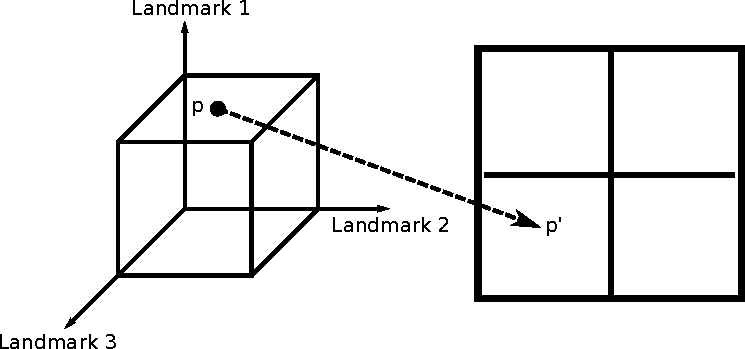
\includegraphics[scale=0.8]{img/algorithms/global_softstate}
% \caption{(left) Position of $p$ in the space of $3$ landmarks. (right) Position
% of $p$ on the map.}
% \label{fig:global_softstate}
% \end{figure*}


%% VM Most of this paragraph on global soft-state rewritten/restructured.
%% Have a look...

\emph{Global Soft-State} \cite{XTZ2003} builds a global view to help nodes
choose shorter routing paths. To generate the proximity information, it 
combines the landmark binning method with small
scale distance probes to reveal the properties 
of the underlying network. 
%Figure \ref{fig:global_softstate} presents the landmark
%space and the mapping of the position of the nodes.

This global view of the network state is used by organizing it into ``maps'' for
regions of the overlay, that are strategically placed
across the network and made available to any node. The notion of a
region is a well defined property for structured \p\ networks and can be part of
the Cartesian space in overlays like \emph{eCAN}~\cite{xu_ecan_2002} or a set of
nodes sharing a particular prefix in overlays such as
\emph{Pastry}~\cite{antony_pastry_2001}. Moreover, a node may appear in a maximum
of $log(N)$ such maps.

Direct access to this information, also coined \emph{soft states}, helps nodes
find the best way to route their messages, while a publish/subscribe mechanism
allows them to get notified on dynamic network changes.

%%
Although this approach does reduce the routing latency to far nodes, it
can become expensive as it is 
possible to end up with a very large number of regions
each of which has to maintain a map. 
The fact that a peer may appear in multiple
such maps points into additional traffic for probing and notifications
and so renders the approach not scalable \cite{RGJZ2004}. 
Moreover, to refine measurements
additional inner-bin measurements are needed~\cite{WZS2004}.
Also, improvements within a region can be minimal as there exists
limited knowledge about neighboring zones.
%%
%%%%%%%%%%%%%%%%%%%%%%%%%%%%%%%%%%%%%%%%%%%%
%%
%% COMM Removed most of the paragraph below which 
%%		contains info that we cannot back
%%
%% Rescanned papers and wrote the paragraph below.
%% DO NOT PERMANENTLY DELETE!
%%
% Unfortunately, maintained of several host states at different layers,
% renders any content migration a costly process. Additionally, the method does
% not make any continuing effort to remap
% the overlay structure after nodes successfully join resulting into poor
% adaptation to changing conditions. Although this approach greatly reduces the
% routing latency to far nodes, it is unable to dynamically identify nodes that
% are close to routers and gateways in order to construct the secondary overlay.
% Nevertheless, static recognition of such nodes is currently done based on BGP
% reports and pre-chosen landmarks, sacrificing the self-organizing attribute of
% traditional DHTs.
%
%
% TODO: SOME DISCUSSION
%
% Xu \textit{et al.} \cite{XTZ2003} state that there are three ways
% generating proximity information
%\begin{itemize}
% \item Expanding Ring Search\\
%Expanding ring search can be of two forms. First it can utilize the multi-cast
%infrastructure in the underlying network in order to emit its messages.
%Unfortunately such infrastructures are not widely deployed thus the
%implementations of this way of generating proximity information is limited to
%blindly flooding the neighborhood to obtain reasonable results.
%
% \item Heuristics\\
%Heuristics are used in order to reduce the blindness of the expanding ring
%search and make realizations more efficient and effective. Unfortunately a
%common problem of all heuristic approaches is the local minimum pitfall in
%which
%the search might be caught into.
%
% \item Landmark Binning\\
%Landmark clustering is based on the view that nodes with similar distances to a
%set of predefined well-known landmark nodes are pretty likely of being close to
%each other. But this approach has its weaknesses as well, such as the fact that
%is a rather coarse grained approximation, therefore not particularly well
%suited
%for differentiating nodes within close distance to each other.
%
%\end{itemize}
%
%
%
% TODO: IN PAPER INTRODUCTION A DISCUSSION ABOUT
%TOPOLOGY-AWARE CAN
%
%Techniques to exploit topology information in overlay
%routing include geographic layout, proximity routing and
%proximity neighbor selection [3]. With geographic layout
%such as topology-aware CAN [12], the overlay structure is
%constrained by underlying network topology. This tech-
%nique, unfortunately, can create uneven distribution of
%nodes in the overlay, increasing the chances of overloading
%nodes and rendering the maintenance cost formidable. Our
%study shows that, for a typical 10,000-node topology-aware
%CAN, 5% nodes occupy 85-98% of the entire Cartesian
%space, and some nodes have to maintain 450-1500 neigh-
%bors. In Proximity routing, physical topology is not consid-
%ered when constructing the overlay.
%
In terms of our $3$ stated criteria, the approach fares as follows:
\begin{center}
{\footnotesize
\begin{tabular}{ccc}
\emph{Efficiency} & \emph{Overhead} & \emph{Scalability} \\
\hline
% Unable to identify nodes that are close to routers but it can reduce routing
% latency to far away node by approximately 50-75%.
medium &
% maintenance of node states, subscriptions and notifications need global
% overview of the overlay resulting in high control overhead
high &
% Statically implemented sacrificing the decentralized nature of DHTs and
% thus poorly scaling. Also we can end up with a very large number of regions.
% Because of the fact that a peer may appear in multiple
% such maps we can conclude that additional traffic for probing and notifications
% renders the approach does not scalable.
low
\end{tabular}
}
\end{center}

%%%%%%%%%%%%%%%%%%%%%%%%%%%%%%%%%%%%%%%%%%%%%%%%%%%%%%%%%%%%%%%%%%%%%%%%%%%%%%%%
% \subsubsection{Mithos}

%% VM Whole paragraph rewritten

%% VM: PREVIOUS COMMENTS BELOW REGARDING PREVIOUS VERSION
%%AD in general some mention of the mismatch problem must be made right???
%%		so that a reasonable connection can be established...
%%AD what is the quadrant??? Hugh???

%%AD ref?? (σ.σ. GPSR protocol)

%%AD the above 5-6 lines sounds impressive but there is little help 
%%	for the average ignorant reader.. what is perimeter walk in 
%%	general? how quadrants are formed? What is their relationship? 

%%AD what is GNP??? How did it "land" here???

\emph{Mithos}~\cite{WR2003} ensures that neighbouring nodes in the overlay are
close also in terms of the underlying layer by integrating proximity layout
and proximity routing overlay optimizations.

During bootstrap, an incoming peer $J$ obtains from a bootstrap node a set of
candidate peers to establish links with. 
Subsequently, the node works iteratively to identify peers that minimize
a given metric (i.e., network delay).
The process stops when no additional peers complying with the above metric 
can be found. 
% 
% and iteratively
% probes for minimizing distances, based on a given metric (i.e., network delay)
% and concluding when no further refinement can be achieved. 
To tackle the local
minima problem that such a gradient descent method suffers from, Mithos probes
nodes within a $2$-hop radius from the current node that helps minimize
the distance before concluding the process.

$J$ is then assigned a synthetic \emph{ID} that
represents the state of minimum distance from its close-by $2$-$d$ neighbourhood as
this was discovered during the aforementioned phase. % iterative selection phase.
The benefit of adopting synthetic coordinates is that distance computations
among nodes can be done in the \emph{ID} space without requiring physical
measurements. 
Mithos proceeds then to designate $J$'s closest neighbours as 
previous steps do not reveal with certainty which these nodes are.
%%
Using Mithos \emph{quadrant-based} mechanism,
$J$  divides the $2$--$d$ space of neighbours in four regions and 
subsequently, establishes a link 
to the closest neighbor in each quadrant of the plane. 
% With peer $J$ dividing the plane into four regions,
% the \emph{quadrant-based} mechanism Mithos employs, suggests that the node
% establishes a link to the closest neighbor in each quadrant of the plane. 
%%
It does so, by starting from a known node in the neighbourhood
and scanning towards all quadrant borders ~\cite{KK2000,R2002}. 

A noted Mithos limitation is that the protocol cannot effectively
handle dynamic arrivals and departures from the network~\cite{RGJZ2004}. 
\cite{CCRK2004}~points out extensive probing for Mithos to determine 
distances and less accurate proximity results compared to other
virtual coordinate systems. The last issue  has been also attributed
by~\cite{WSS2005} to the iterative neighbor selection process that is 
reportedly prone to premature termination at local minima.
%%
\cite{cox_vivaldi_2004} argues that elements of the protocol's
synthetic ID generation require a centralized implementation 
affecting Mithos' scalability.
%%%%%%%%%%%%%%%%%%%%%%%%%%%%%%%%%%%%%%%%%%%%%%%%%%%%%%%%%%%%%%%%
In regard to the $3$ criteria, \emph{Mithos} stands as follows:
\begin{center}
{\footnotesize
\begin{tabular}{ccc}
\emph{Efficiency} & \emph{Overhead} & \emph{Scalability} \\
\hline
% It has very good results in reducing communication latency among peers but its
% efficiency is being constrained by the fact that the proximity is calculated
% at bootstrap, assigning virtual coordinates that are used throughout of a
% nodes life cycle and thus the overlay is not adapting to a high-churn
% environment.
medium &
% Incremental probing is applied in quadrants and in two-hop distance at each
% step that does not generate a lot o control overhead.
medium &
% It is constrained by the fact that the protocol does not respond to dynamic
% peer arrivals and departures
low
\end{tabular}
}
\end{center}

%%%%%%%%%%%%%%%%%%%%%%%%%%%%%%%%%%%%%%%%%%%%%%%%%%%%%%%%%%%%%%%%%%%%%%%%%%%%%%%%
% \subsubsection{LAPTOP}
%
%%AD what is the nature of the "structure" overlay here???
%% VM the structure is that it is organized as a tree hierarchy.
\emph{LAPTOP} \cite{WLH2007} organizes the overlay 
into a tree-based hierarchy so that 
hops required during message routing be reduced and 
maintenance overhead be minimized.
A caching scheme is also used so as
to further lower routing table update costs. 
It is theoretically shown that 
\emph{LAPTOP} routing path length is bounded by $O(log_d(N))$ and node
joining and leaving in the overlay network is bounded by
$O(d*log_d(N))$ hops in a balanced overlay tree with $N$ representing the
number of nodes and $d$ the maximum degree of each node (i.e., number of links). 
\emph{LAPTOP} adopts the geographical layout approach  
and constructs its layout in a self-organizing and 
efficient fashion. 
The physical distances are estimated
with round trip times to a few existing nodes in the overlay network.
%%
Each node is assigned a dot-formatted address (e.g., 1.3.4) with
each octet ranging from $1$ to $d$.
The assignment process is done by appending a unique octet 
to the address of the parent of each node, while
the root node is assigned address $1$.

%The protocol is based on four definitions.
%\begin{enumerate}
% \item The amplitude of all possible measured RTTs is divided into intervals.
%  Each node measures its distance to its parent and is assigned a label $L_i$
% where $i$ denotes the configurable RTT interval in which the measured distance
% falls into. A special kind of node, the root, is initially assigned the $L_1$
% label and maintains (as all $L_1$ nodes do) a list of other $L_1$ nodes in the
% overlay.
% \item Any node can have children with level lower than theirs, except an
%  $L_{max}$ node which can only have $L_{max}$ level children and only in the
% case when its parent has reached its maximum degree.
% \item Each node is assigned a dot-formated address (e.g 1.3.4). Each octet
% ranges from
% $1$ to $d$, where $d$ is the maximum degree of the nodes. The assignment
% process
% is done by appending a unique octet to the address of each nodes parent, while
% root node is assigned address $1$.
% \item For any descendant node $Y$ of a node $X$, the measured distance among
%  each other, must always be less than the lower bound of the RTT interval
% denoted by $X$'s label.
%\end{enumerate}
%

\emph{LAPTOP}'s routing scheme is similar to the 
longest-prefix \emph{IP} matching scheme. 
At each forwarding hop, a message travels up the tree 
until the first common ancestor of both source and destination nodes 
is reached and then, the message starts descending towards its target. 
During tree traversals, special entries in the routing tables
are maintained to increase routing efficiency and achieve finer--load balance.
These special entries constitute the \emph{routing cache} which enables a node
to forward a message to a better 
longest-prefix match than that of its direct ancestor;
this yields a quicker and more cost--effective step through the overlay towards
the destination. 
To improve scalability, the number of child nodes and the
size of the routing cache are limited. 
To contain maintenance costs, \emph{LAPTOP} employs 
a simple \emph{heartbeat}-based regime in which 
a parent is responsible for the monitor of its own children.
%%%%%%%%%%%%%%%%%%%%%%%%%%%%%%%%%%%%%%%%
%
%The new comer $N$ locates the root node and the later responds with a list of
%  $L_1$ nodes. $N$ then probes each of the $L_1$ nodes in search for the
% closest one. If the measured RTT to the closest $L_1$ falls into the first
% interval then the new comer becomes a $L_1$ node as well. Otherwise node $N$
% sets the closest $L_1$ node as its potential parent node. This potential
% parent becomes the actual parent if it does not have any other children. If it
% has, $N$ gets a list of these $L_i$ nodes and by measuring the RTT to each of
% them tries to spot a new potential parent in order to repeat the above
% process.
%
%
% At join process the new coming node is assigned its level label as well as its
% address by its parent node. Additionally, it initializes its routing table
%(with normal and caching entries) as it traverses the overlay in search for
%its parent node.  During a graceful departure, the referred node checks for
%children in the overlay. If it does not have any, it simply notifies its
%parent and leaves. If it has, it selects the child node with the lowest
%round-trip time to it in order to take its place so that the locality
%property is preserved. On the other hand, in the case of an arbitrary
%failure, after the children of the failed node detect their parent's absence
%(through the aforementioned heartbeat mechanism), they start emitting special
%messages to their grandparent node (the address of which is stored during
%join process}. In case of no response from the grandparent node, the children
%invoke the joining process to detect their new parent node.The parent of the
%failed node, aggregates the notifications from the above children nodes for a
%period of time, and then chooses the one with the lowest level label as the
%takeover node. Potential ties are broken by favoring the lower RTT. The
%parent of the failed node, finally informs accordingly all the children about
%the change in the hierarchy.
%%%
%
%%%%%%%%%%%%%%%%%%%%%%%%%%%%%%%%%%%%%%%%%%%%%%%%%%%%%%%%%%%%%%%%%%%%%%%%%%%%%%%%
%
% TODO: HERE STRUCTURED LANDMARK BINNING APPROACH LIES
%
%Assuming a structured approach based on CAN\cite{ratnasamy_can_2001} and $m$
% landmark nodes. The coordinate space is then partitioned into $m!$ equally
%sized portions, each corresponding to a single ordering of the landmarks. To do
%this, the first dimension is divided into $m$ areas each of which is further
%divided (second dimension) into $m - 1$ sections and so on. Having set this $m$
%dimensional space, at joining time, a node measures the delay to the set of
%landmarks in order to determine its associated bin and thus position itself in
%that portion of the coordinate space associated with its landmark ordering.
%Even though this scheme can
%
\emph{LAPTOP}'s behavior for the $3$ criteria stands as follows:
\begin{center}
{\footnotesize
\begin{tabular}{ccc}
\emph{Efficiency} & \emph{Overhead} & \emph{Scalability} \\
\hline
% It minimizes routing length, but may suffer load imbalance since nodes higher
% in the tree hierarchy are more likely to route most of the messages in the
% overlay.
medium &
% Heartbeat approach incurs extra control overhead to the network. Fortunately
% involves only the parent and the children of the departing/failing node.
% nodes.
low &
% Seems to scale nicely from 10K- to 1M-node testbeds.
high
\end{tabular}
}
\end{center}


%###############################################################################
%###############################################################################
%###############################################################################
%       PROXIMITY ROUTING
%###############################################################################
%###############################################################################
%###############################################################################


%%%%%%%%%%%%%%%%%%%%%%%%%%%%%%%%%%%%%%%%%%%%%%%%%%%%%%%%%%%%%%%%%%%%%%%%%%%%%%%%
% \subsubsection{Proximity in Kademlia}
% Before discussing {\em Proximity in Kademlia}, it would be helpful to briefly
% summarize the highlights about the {\em Kademlia} protocol. {\em Kademlia}
% \cite{maymounkov_kademlia_2002} is a distributed hash table (DHT) based
% protocol for \p\ networks, which uses an iteration based lookup algorithm. The
% protocol uses the standard $160$ bit ID system for nodes and locates the nodes
% in a prefix binary tree, where IDs are used as prefixes. The iterative lookup
% operations are done over this prefix binary tree, which converges to
%logarithmic
% lookup times. The ID's are assigned randomly, therefore in Kademlia, there is
%no
% proximity control, which results in inefficient use of the underlying network
% during lookup and retrieve operations.

In order to optimize the underlying network use,
\cite{KLKP2008} introduces proximity
controls over the \emph{vanilla Kademlia}~\cite{maymounkov_kademlia_2002} 
protocol's random \emph{ID} assignment.
% The work in this paper
% can also be considered as a more generic study of incorporating proximity into
% iterative lookup algorithms.
In its quest to improve routing performance, the overlay uses 
a cost ``yardstick'' (i.e., metric) provided by the underlying network.
% The overlay tier improves its routing performance using a cost--metric that is
% provided by the underlying tier. 
Such cost information can be acquired by:
\begin{inparaenum}[\itshape i\upshape)]
  \item measuring previous lookups,
  \item exchanging or jointly-computing measurements with others, or 
  \item using a local database to look--up information.
\end{inparaenum}

\cite{KLKP2008} exploits two routing techniques: 
\emph{proximity routing selection (PRS)} and 
\emph{proximity neighbor selection (PNS)}.
%%
In \emph{PRS}, the goal is to choose the best next hop while routing a message.
\emph{Kademlia} always selects the closest--node 
with respect to the \emph{XOR} metric~\cite{maymounkov_kademlia_2002}.
With \emph{PRS} in place however, \emph{Kademlia} may also choose 
the node that exhibits the smallest routing cost; in this way, 
it balances a trade-off between the logical overlay and 
actual underlying distances.
%%AD rephrased as above.. the "underlay" I am not sure what it is...
%  but with proximity routing, Kademlia should also choose the node
% that exhibits the smallest underlay metric cost, balancing a trade-off between
% the overlay and underlay progress distances.
%%
%% VM rephrased to not contain the word "underlay". Clean up comment block if OK.
%%
In \emph{PNS}, on the other hand, the goal is to keep peers 
with the least routing cost in the routing table. 
%%AD WHAT is this "least contact cost"?? Sounds funny! CHECK
%% VM rephrased to not contain the word "contact". Clean up comment block if OK.

%%
%% VM Commenting out since this info is not that important I believe
%%
%As \emph{Kademlia} continually learns about new
%peers via incoming requests and an iterative lookup process, 
%%%AD what is this iterative lookup process???
%no specialized algorithm is required for searching for 
%more cost-effective peers 
%and the system simply goes for the best peers ``seen'' thus far.

\emph{Kademlia} proximity injection improves 
locality of connections among peers.
To enhance traffic locality, the use of 
{\sl MaxMind GeoIP} database\footnote{\url{http://www.maxmind.com}} 
is suggested to form clusters of nearby peers.
To this end, Vivaldi coordinates~\cite{cox_vivaldi_2004} could be 
also used as an alternative for morphing locality. 
\cite{KLKP2008} however suggests that the clustering approach 
when combined with \emph{PRS}/\emph{PNS} helps contain 
$40\%$ of messages within an \emph{ISP} and allows only a $6\%$ 
to go through the backbone.
The behavior of \cite{KLKP2008} with respect to the stated criteria is deemed as follows:
%%
\begin{center}
{\footnotesize
\begin{tabular}{ccc}
\emph{Efficiency} & \emph{Overhead} & \emph{Scalability} \\
\hline
% Uses static information to cluster nodes which is not the most efficient
% approach in dynamic systems
% PNS reduces lookup latencies by 66\% compared to POK
medium &
% 
medium &
% MaxMind is commercial and cannot be used by FOSS P2P systems. Trying to
% expose information from P2P client can result in security issues.
medium
\end{tabular}
}
\end{center}

%%%%%%%%%%%%%%%%%%%%%%%%%%%%%%%%%%%%%%%%%%%%%%%%%%%%%%%%%%%%%%%%%%%%%%%%%%%%%%%%
% \subsubsection{CHOord considering Proximity on IPv6 (CHOP6)}

%%AD how does CHOP6 helps with the mismatch problem??
%% VM rewrote the whole part to answer this question
%% By and large, rtt measurements and id assignment help choose the next best
%% hop during routing that is i) toward the key and ii) has small cost
%% either in terms of explicit RTT or implicit RTT (taking regional/national
%% hops as a proxy of proximity - international RTT > regional RTT > national RTT)

\emph{CHOP6} \cite{MT2007} is a Chord-variant DHT that exploits
{\sl IPv6} address format as well as available \emph{RTT} information to 
enable proximity estimation among peers during message routing.
%%
Similar to \emph{Chord}~\cite{stoica_chord_2001}, 
\emph{CHOP6} uses a finger table with each entry now holding $k$$>$$1$ candidate
nodes. 
The next hop for a message is selected to be the one closest to the
destination among those $k$ candidate peers. 
This proximity is determined either
by exploiting RTT measurements or, if there is no such information yet 
(i.e., a new peer appears), by
estimating distance on the overlay's ID space. 

When joining the network, each node
receives a $64$-bit \emph{ID}. 
It comprises of a random part and the IPv6 prefix which 
is obtained by hashing the node's IP address and port
number; this combination is deployed in an effort  
to preserve the uniformity of node assignment. 
The prefix in question is based on IPv6's global routing prefix.
As IANA\footnote{\url{http://www.iana.org/}}  
assigns address blocks to regions (RIRs) which are further
distributed at national level (NIRs), the first $32$-bits of the address
can estimate the region or the country the node is connected in. 
Thus, CHOP6's IPv6 prefix ID is used for proximity estimation
if no RTT information is available during routing. 
%%
%
%\paragraph{}
% There are three cases in which a node chooses the next hop according to
% information it possesses.
%\begin{itemize}
% \item When no information about RTT is available candidate next hops, the
%  sender just selects a node in the finger table entry which shares the longest
% prefix with the destination.
% \item There is another possibility that after some communication with other
%  nodes, the source node should know of the RTTs to some of the nodes in finger
% table entry. In this case, the source node chooses the one with the smallest
% RTT with probability $p$. If there is a node with no measured RTT then the
% sender can select such a node with probability $1 - p$
% \item In this last case the source node has already communicated with all
%  candidate node in the finger table entry. Thus, the node selects the node
% whose RTT is the smallest with probability $p$, the one with the second
% smallest with probability $q$ and so on, where $0 \leq \ldots < r < q < p < 1$
% and $p+q+r+\ldots \leq 1$
%\end{itemize}
%
With respect to the $3$ qualitative criteria, \emph{CHOP6} stands as follows:
\begin{center}
{\footnotesize
\begin{tabular}{ccc}
\emph{Efficiency} & \emph{Overhead} & \emph{Scalability} \\
\hline
% Simple approach that exploits proximity but it is coarse grained and thus not
% efficient.
low &
% Its static nature imposes low overhead to the network
low &
% IPv6 is still not widely applied and supported.
medium
\end{tabular}
}
\end{center}


%%%%%%%%%%%%%%%%%%%%%%%%%%%%%%%%%%%%%%%%%%%%%%%%%%%%%%%%%%%%%%%%%%%%%%%%%%%%%%%%
% \subsubsection{T2MC}

%%AD a better connection with the mismatch problem has to be made... 
%%		.. in the form of 1-2 lines (or short statements). 
%%
%% VM Added some extra lines and restructured the text
\emph{T2MC}'s~\cite{SLCGZ2008} objective is to diminish the redundant multiple
messages that may unnecessarily cross autonomous system (\emph{AS}) boundaries.
The latter represent links that are the costliest to ISPs and hence, 
mininizing topology mismatches  greatly affects pertinent operational expenditure.
%%
To achieve that, each node exploits the stable structure of
the Internet routers to help solve a clustering problem. 
The algorithm uses {\sl traceroute}-logs to detect inter-\emph{AS} boundaries 
and clusters peers to either nearby or 
far-away groups by applying a customized $k$-mean classification ($k=2$).
%%
When joining the network, the peer randomly picks an IP and uses
traceroute and selects the routers with
minimum and maximum latencies in the above {\sl traceroute} path 
as initial centroids for the ``nearby'' and ``far-away'' sets respectively.
Following an iterative procedure, the node comes up with the two sets 
demostrating minimum intra-set latency variance.
At this stage, routers in the ``far-away'' set are not considered critical.
%%
%%AD skipping the details???? JUST CHECK
% Skipping the details of the algorithm, it picks the routers with
% minimum and maximum latencies in the above traceroute path as initial centroids
% for the ``near'' and ``remote'' sets respectively and after some iterations it
% ends up with two sets having the minimum intra-set latency variance. 
%%
% The router from the ``far-away'' set that presents the closest distance 
% from the peer in terms of hops, is designated as beacon.
% Any node portaying dinstance longer that the above is classified 
% as 
% 
% to the peer, in terms of hops, is designated as a beacon.
% Any node whose distance is measured to be longer that the distance 
% between 
% 
% The router with the minimum hops in the ``remote'' set is set up as the hop
% threshold and anything above that is classified as the ``remote'' router cluster
% for that peer. 
% Similarly, 
In contrast, the router from the ``near'' set
having the maximum number of hops 
from the just-joining peer is key as it denotes an edge--gateway. 
Peers that share the same edge--gateway or other members in the ``nearby'' 
router cluster are considered intra-\emph{AS} neighbors.
%%AD the final phrase for this is missing! So what??? What is achieved? 1 sentence.

Even though {\sl traceroute}
provides detailed information about the network structure, 
its extensive use may create overhead on the overall network structure. 
In this respect, administrators frequently
disable {\sl traceroute} support on their routers this 
undoubtly affects \emph{T2MC}'s operation.
%%
Although overall experimental results have been encouraging, 
\emph{T2MC} is considered rather coarse-grained as it only
classifies neighbours into two groups \cite{QLZG2009}.
%
%T2MC \cite{SLCGZ2008} uses trace-route logs to detect different autonomous
%systems and cluster close by peers, thus reducing redundant traffic that crosses
%autonomous system boundaries. T2MC uses a customized k-mean classification
%algorithm with $k=2$ to perform the classification, and exploits the stable
%structure of the Internet routers to guide clustering. The peer chooses the
%minimum and maximum Latency results from the trace-route to initialize the
%centroids of two sets. Then the peer calculates, for all hops along its
%trace-routed path, the peer calculates the absolute distance to these centroids
%of both sets and assigns the routers to that centroid with which it has the
%smaller absolute distance. After that, the mean and variance values are
%calculated and if the variance is larger than a predefined threshold then the
%algorithm sets the two latency mean values as new centroids for the two sets and
%loops again. Ultimately peer will end up with two sets having the minimum
%intra-set variance. The peer, then, chooses the router from the second set with
%the minimum hops attribute and sets it as a threshold. The selected router and
%all others whose hops attribute is larger than the threshold are classified as
%\emph{remote} router cluster. The remaining are classified as \emph{near}. From
%the near class, the peer chooses the one with maximum hops attribute as its edge
%router, and registers it along with all near clusters into the DHT of the
%\p\ overlay. As new peers join the network, those that share the same edge
%router or any of the members of the near router clusters, would form a close
%peer cluster. As Edge routers can provide more valuable information than other
%members of the near set, T2MC was designed to prioritize interaction of peers
%and edge gateways.
%
%
% TODO: SOME DISCUSSION
%
%The use of Trace-route as a tool for implementing the distance measuring
%infrastructure raise concerns about its efficiency and scalability. Being,
%primarily, a network diagnostic utility,
% Even though trace-route provides detailed information about the network
% structure, its excessive use creates additional overhead that stresses further
% the overall network infrastructure. This forces network administrators to
% disable its support from the routers they manage, thus jeopardizing the
% effectiveness of the T2MC algorithm.
%
\emph{T2MC} fares as follows:
%%
\begin{center}
{\footnotesize
\begin{tabular}{ccc}
\emph{Efficiency} & \emph{Overhead} & \emph{Scalability} \\
\hline
% The efficiency of choosing close by peers is very good and reported almost
% 65\% better than that of GNP (and thus generally of static landmarking as a
% whole)
high &
% trace-route is a very heavy tool and thus incurs excessive burden to the
% network resources.
high &
% Trace-route is categorized as too heavy-weighted and intrusive for use in a
% larger scale system \cite{RKHS2002}. Additionally, disabling
% ICMP is a common administrative policy for edge sites to enforce security,
% while dumping BGP routing tables\cite{krishnamurthy_bgpclust_2000} is not
% directly available to the application layer.
low
\end{tabular}
}
\end{center}

%%%%%%%%%%%%%%%%%%%%%%%%%%%%%%%%%%%%%%%%%%%%%%%%%%%%%%%%%%%%%%%%%%%%%%%%%%%%%%%%
% \subsubsection{PChord}
\emph{PChord} \cite{HLYW2005} is based on the \emph{Chord DHT} and adds
proximity into its routing mechanism. 
To achieve that, the standard finger table
is augmented with a \emph{proximity list} that contains
nodes in the network found close-by in terms of RTT.
%in this way, the next hop can be decided based on both progress
%towards the key and the physical proximity of the candidate nodes.
%%AD
%% I am not sure about the "best progress" term - what does it really mean???
%% VM changed the above slightly to address the above comment. Generally
%% in DHTs when a node receives a search query for a key that it does not have
%% the data for, it routes the request to that node in its routing table that
%% is closest to the key. That is what I mean with best progress to the keys
%% In topology aware systems and topology aware routing we have the requirement
%% that the next hop should be the closest one which in many cases can be
%% a competing requirement with the best progress to the key requirement I
%% just described. 
In this respect, the next hop during routing can be decided based on both the
direction towards the search key and minimizing the cost of that hop.

When a peer joins the network, its proximity list is empty.
This list is maintained in a heuristic fashion during the node's lifetime.
While a node attempts routing, the next hop is selected
as the closest node to the target key 
from \emph{both} its finger table and proximity list. 
An initial choice for the next hop made out of the finger list 
can be substituted by a shorter one from the proximity list if  
it is both closer to the key and in less physical distance.
This yields an equal or even more efficient routing than traditional Chord.
%% VM
%% Removed the text below that was a rephrasing of one of my own a little
%% bit more below. Hope it is way more clear now.
%%
% As there is always progress towards the target in the \emph{ID}-space,
% \emph{PChord} yields a reduced number of hopes that \emph{Chord}.
%%AD rephrased as above - the 2 last lines of the text below are 
%%		are difficult to decipher... 
% Due to the fact that, with each step, there is always 
% progress towards the target node in the ID space, 
% \emph{PChord} will result in a reduced hop number than
% Chord, since each hop in \emph{PChord} is larger or 
% at least equal in the key space.

Unfortunatelly the overlay maintenance cost is somewhat higher than
\emph{Chord} as additional heart-beat messages are required for
connection verification for the entries of the proximity list. 
Fortunately, such entries represent nodes 
already close-by so the additional cost is kept to a minimum.
However, \emph{PChord} has been reported to exhibit slow convergence speed 
and inefficiency in high-churn environments~\cite{DK2006}.
%%
%%%%%%%%%%%%%%%%%%%%%%%%%%%%%%%%%%%%%
%%
%% VM:
%% Removed this whole chuck since most of it sounded like
%% repetition of the rest of the text below after all.
%% Please review and remove if you aggree.
%%
% Passing through proximity links, in the underlying network, 
% means reduced routing cost. 
% Moreover, if the number of entries in the proximity list is the same
% as the number of network partitions, 
% \emph{PChord} prevents hops from jumping in and
% out of network partitions the current node belongs to.
% On one hand, 
% \emph{PChord}’s advantageous  points are that 
% its routing attains fewer overlay hops, 
% it crosses network partition(s) only once by following proximity links
% and it maintains the light-weight maintenance cost of \emph{Chord}.
% On the other, \emph{PChord} exhibits slow convergence speed 
% and inefficiency in high-churn environments~\cite{DK2006}.
% %%AD rephrased what is below as above... 
% % \emph{PChord}’s advantages include the fact 
% % that the main routing optimizations are of
% % less overlay hops, following proximity links and crossing the same network
% % partition only once along a routing path while in the same time keeping Chord's
% % light-weight maintenance cost. 
% % On the other hand, it exhibits slow convergence
% 	% speed and inefficiency in a high churn environment \cite{DK2006}.
%%%%%%%%%%%%%%%%%%%%%%%%%%%%%%%%%%%%%%%%%%%%%%%%%
\emph{PChord} qualitatively behaves as follows:
\begin{center}
{\footnotesize
\begin{tabular}{ccc}
\emph{Efficiency} & \emph{Overhead} & \emph{Scalability} \\
\hline
% Small decrease in needed overlay hops per object publishing but rigid in
% high churn environments.
medium &
% The are heartbeat mechanism for both finger table and proximity list adds a
% burden to the network by default. But the overall overhead is decreased as
% the proximity list becomes longer.
medium &
% Improvement of routing is achieved with more object pointers helping to
% shorten the routing path of object querying. When the distance of query source
% to target is far away both Chord and PChord achieve the average hop number to
% not increase.
medium
\end{tabular}
}
\end{center}

%%%%%%%%%%%%%%%%%%%%%%%%%%%%%%%%%%%%%%%%%%%%%%%%%%%%%%%%%%%%%%%%%%%%%%%%%%%%%%%%
% \subsubsection{AChord}
\emph{AChord} \cite{DK2006} exploits IPv6's \emph{anycast} mechanism to
relieve the protocol from complex joining procedures,
harness network proximity and achieve high routing efficiency. 
When sending a message to an IPv6 anycast group, 
the originator accomplishes this delivery by interacting with
the physically closest node in that group~\cite{M2002}.
Thus, \emph{AChord} organizes all nodes participating
in the overlay network into a single anycast group. 
An arriving peer is automatically forwarded to the physically 
nearest node for
bootstrapping; this curtails the need to explicitly maintain participants
and the effort of locating the physically nearest. 
%%

The \emph{ID} of an incoming node is computed based on 
both the identifier of the bootstrap node 
and the bootstrap's predecessor;
this is  done in a way that the \emph{ID} of the 
incoming peer is positioned \emph{between} the two identifiers mentioned above. 
After joining, a \emph{finger} table is created ala \emph{Chord}. 
Moreover, an \emph{adjacency table} maintains 
information about the $k$ closest--known peers. 
%%
The routing decision takes place in a way reminiscent to \emph{Chord}
and uses both adjacency and finger tables.
%%
\emph{AChord} behavior has as follows:
\begin{center}
{\footnotesize
\begin{tabular}{ccc}
\emph{Efficiency} & \emph{Overhead} & \emph{Scalability} \\
\hline
% good routing efficiency but no adaptation to high churn environments.
medium &
% Relieves the system from joining overhead and topology aware ID construction
% but doubles the information needed to be stored and maintained by the
% introduction of adjacency table
medium &
% assumes the operation of ideal underlying any-cast mechanism (meaning that
% outside messages are always routed to the nearest node which in the current
% Internet, this is not always feasible. Moreover, is designed on the basis of
% IPv6 protocol which is not widely operational yet.
medium
\end{tabular}
}
\end{center}

%%%%%%%%%%%%%%%%%%%%%%%%%%%%%%%%%%%%%%%%%%%%%%%%%%%%%%%%%%%%%%%%%%%%%%%%%%%%%%%%
% \subsubsection{Chord6}
\emph{Chord6}~\cite{XZHL2005} is another \emph{Chord}-variant that
uses IPv6's  hierarchical features to create 
a substrate that reduces inter-domain traffic among service providers. 
The key difference between
\emph{Chord6} and \emph{Chord} lies on the identifier definition. 
The adopted approach is deemed as easily portable to other 
\emph{DHT}s including \emph{CAN}, \emph{Pastry} and \emph{Tapestry}. 
%%
\emph{Chord6}'s identifier contains two parts: 
the higher bits are obtained by hashing the
node's IPv6 address prefix (of specific length), 
while the remaining lower bits of the identifier 
is the hash-value of the remaining of the IPv6 address. 
%%
As a result, nodes in a domain are mapped 
onto a continuous key space on the overlay network;
the latter avoids unnecessary message--forwarding across different
service providers and helps minimize overall routing cost.

\emph{Chord6} does reduce the average 
length of hops traversed
% system path length 
to be logarithmically proportional to the number 
of available domains instead of the number of participating peers. 
Due however to the large number of Internet
domains and the possibility of occasionally having only 
a small number of peers within each domain,
\cite{DK2006} challenges the approach's scalability and efficiency.
%%
Overall, the approach fares as follows:
\begin{center}
{\footnotesize
\begin{tabular}{ccc}
\emph{Efficiency} & \emph{Overhead} & \emph{Scalability} \\
\hline
% Can reduce inter-domain average path length but even though nodes in the same
% domain would have close identifiers, nodes in two close domains may have very
% different ones reducing the overall efficiency of the approach in general when
% considering inter-domain average path length. No active adaptation mechanism
% for high churn environments.
low &
% The construction of the identifier space is done at node join and in an
% independent fashion involving the application of two hash functions meaning
% resulting in low overhead stress to the network and its nodes.
low &
% Is designed on the basis of IPv6 protocol which is not widely operational yet.
low
\end{tabular}
}
\end{center}

%###############################################################################
%###############################################################################
%###############################################################################
%       PROXIMITY NEIGHBOR SELECTION
%###############################################################################
%###############################################################################
%###############################################################################

%%%%%%%%%%%%%%%%%%%%%%%%%%%%%%%%%%%%%%%%%%%%%%%%%%%%%%%%%%%%%%%%%%%%%%%%%%%%%%%%
% \subsubsection{DHT-PNS}
A proximity neighbor selection scheme functioning atop 
the \emph{Chord DHT} is introduced in~\cite{DLTZZ2006}.
Its key objective was to group physically-close nodes as 
neighbors in the \emph{DHT} table while exploiting proximity information.
To detect proximity, virtual network coordinates for 
peers are used with the help of the Vivaldi protocol~\cite{cox_vivaldi_2004}. 
The virtual coordinates are then used to help map nodes to 
the identifier--space of the \emph{DHT}.
%%
The space in question is partitioned using a 
\emph{concentric circle clustering scheme} where successive cycles of
radiuses $\rho$, $2\rho$, $3\rho$ and so on, are constructed. 
The formed annuluses are then divided into 
$2\chi-1$ \emph{sectors}, where $\chi$ denotes the
sequence number of the annulus starting from $\chi = 1$ 
for the center cycle. 
In this way, 
\cite{DLTZZ2006} prove that each sector
This characteristic favors a more load--balanced clustering operation
should we assume uniform node distribution.
Every sector in this $2d$ space is mapped to 
a unique \emph{region} in the \emph{DHT} space forming a
multi-layer node identifier space.  
Consequently, nodes from the same
sector are mapped to the same region as well, 
preserving their proximity relationship. 

Individual elements are uniquely mapped to the identifier--space,
allowing logarithmic lookup operations with high 
probability on \emph{Chord}. 
To this end, 
a node can obtain its \emph{DHT} key and its region key, 
in a fully distributed manner, just by applying a consistent hash function. 
The node can then communicate with the region's
master node called \emph{Cluster Node (CN)} which 
is responsible for clustering 
the nodes belonging in the same sector or 
region with that of the node at hand. 
%%
The node registers to its corresponding region  and publishes
its information, through the special peer \emph{CN};
the peer can also ask \emph{CN} for other
nodes that have previously joined the region to enhance 
the peer's neighbor set for future routing table optimization.
%
If no other nodes are found within the region, 
the search is expanded to neighbouring regions.
%
%% VM rephrase the one bellow as above in a super compact form
%%AD the one below is not a parse-able sentence!!! What does it say???
%%%		restrict the length of your sentences to say at most 2.5 lines!
%Even in the case when no
%neighbor is detected in the current region, the search is expanded to adjacent
%regions and towards an upper layer identifier space until one is found or the
%first layer reached. Simulations suggest that the scheme has good convergence
%property of the delay distribution and good optimizing performance.
%
%
%%AD up to here the text in this second paragraph for Chord DHT remains 
%%%%%		... rather cryptic - does need work and better connection 
%%%%%		with the 1st paragraph...
%%
Even though scaling appeared promising, only limited 
simulations were carried out with configurations involving up to 2,048 nodes.
Moreover the approach assumes uniform node distribution which
is not always the case, especially in a synthetic coordinate system.
%%
\emph{Chord DHT} fares as follows in reference to the stated $3$ criteria:
\begin{center}
{\footnotesize
\begin{tabular}{ccc}
\emph{Efficiency} & \emph{Overhead} & \emph{Scalability} \\
\hline
%
medium &
%
medium &
%
medium
\end{tabular}
}
\end{center}



%%%%%%%%%%%%%%%%%%%%%%%%%%%%%%%%%%%%%%%%%%%%%%%%%%%%%%%%%%%%%%%%%%%%%%%%%%%%%%%%
% \subsubsection{Quasi-Chord}
\cite{SZ2008} proposes \emph{Quasi-Chord}, a \emph{Chord}-based network that
constructs its overlay network while attempting to match the underlying 
network topology.
The overlay creation follows $3$ stages:
first, each host acquires its coordinates in
a geometric space using the \emph{Global Network Position (GNP)} protocol
\cite{ng_gnp_2001} and a set of landmarks.
Second, using the \emph{Cantor} space--filling curve, 
the $2$-dimensional is converted to $1$-dimensional space. 
The latter is employed in the third and final stage to build 
the \emph{Quasi-Chord} circle according to the host's \emph{Cantor} value. 
Physical proximity is thus denoted by \emph{Cantor} value proximity. 
The \emph{Chord} cycle is constructed by sorting nodes in 
ascending order.
%In \emph{Quasi-Chord},
%each node stores $2$ finger tables; one clockwise and one counter-clockwise.
%%AD what is the purpose of this? efficiency to go back and forth???
% VM not relevant to the topology awareness so I removed the sentence above
%%
%
%In the following paragraphs, these steps are further discussed.
%
%\paragraph{GNP coordinates}
%First of all the host must be positioned in the geometric space. The algorithm
%  models the \p\ network with a well defined distance function in such a way,
% it can predict, with high accuracy, the distance between any two points in the
% space by just evaluating the output of the distance function on the
% coordinates of these points. This is accomplished with the \emph{global
% network position (GNP)} protocol which\begin{inparaenum}[\itshape i\upshape)]
%  \item creates a reference set of $N$ landmark nodes so as to minimize the
%  error of ICMP measured distances and coordinate computed ones between them,
% and then
%  \item each host is able to measure its round-trip times to the $N$ Landmarks
% in order to compute its own coordinates.
%\end{inparaenum}
%
%\paragraph{Cantor SPF}
%After the $2$-d coordinates are set, in the next stage of the algorithm, each
%  participating peer is assigned a Cantor value, according to the application
% of a \emph{space filling curve} on the coordinate space. (TODO: add figure).
% This results in the conversion of the $2$-dimensional space to a
% $1$-dimensional Cantor space that can more easily be more mapped to the Chord
% hierarchy.
%
%\paragraph{Quasi-Chord construction}
%As can intuitively be inferred by observing the Cantor chart, close-by nodes in
%  the physical layer, are more likely to have similar Cantor values. This
% attribute is exploited in order to construct a topology-aware identifier space
% for the Chord DHT. The cycle is constructed by sorting nodes in ascending
% order. Each host maintains 2 finger tables, one for clockwise and one for
% counter-clockwise stepping. This helps with the connectivity of the network
% because its not allowed to connect the first node with the last one since this
% will incur heavy traffic to the later\footnote{After all their Cantor values
% denote that they are actually the furthest of each other.}.
%
%
%
% TODO: SOME DISCUSSION
%       NEEDS DOUBLE-CHECK
%
%The disadvantage of the algorithm is that the coordinate assignment in the
%  first stage is backed by a not fully distributed landmark-based algorithm.
% Moreover the Quasi-Chord model build-up is making an indirect assumption of a
% maximum number of allowable hosts since it is constructed. Last but not least
% the doubling of the required routing information which needs to be created and
% maintained is an additional negative point to the efficiency and the
% scalability of the algorithm.
%
%%
\emph{Quasi-Chord} qualitative behavior has as follows:
\begin{center}
{\footnotesize
\begin{tabular}{ccc}
\emph{Efficiency} & \emph{Overhead} & \emph{Scalability} \\
\hline
% The algorithm shows to reduce end-to-end delay as well as not produce
% duplicates of messages.
medium &
% The overhead is more compared to vanilla chord since mapping of 2-dimensional
% space to 1-dimensional with Cantor SPF adds some extra burden in time
% complexity. Also the addition of the counter-clockwise finger table doubles
% the data, per se, needed to be stored and maintained.
high &
% The GNP system is a static landmark approach making things not fully
% distributed and thus constrain the model's scalability.
medium
\end{tabular}
}
\end{center}

%%%%%%%%%%%%%%%%%%%%%%%%%%%%%%%%%%%%%%%%%%%%%%%%%%%%%%%%%%%%%%%%%%%%%%%%%%%%%%%%
% \subsubsection{IP-based Clustering (IPBC)}
\emph{Proximity neighbor selection} algorithms often 
use probing to detect proximity. 
However, such methods suffer by imprecisions often due to network overload.
IP-based clustering or \emph{IPBC}~\cite{KM2007} uses IP address prefixes
($16$~bits for IPv4) to detect proximity.
Such proximity information 
% (IP addresses of network participants) 
can be easily stored in the DHT itself.

Each peer in the overlay has a unique \emph{ID} and and an IP address to
characterize it. 
To publish itself, the peer hashes a fixed-length prefix of 
its IP to obtain a key and stores the resulting \emph{ID} and IP 
in the DHT. 
Newly joining nodes with the same {\sl IP} prefix 
can, thus, query the \emph{DHT} and readily identify all 
neighbors with the same prefix. 
Nodes periodically update their entries in the \emph{DHT} 
by removing those who leave or have timed-out.
%%

The overhead of the algorithm is very low as proximity detection requires only
a comparison of prefixes. On the other hand, the efficiency of the proximity
is caught into a vicious cycle with the storage space needed for \emph{DHT} 
object publishing.
Moreover, its static nature assumes high correlation of common IP prefix
length of participating peers and latency (with no other measurements),
which might not always be the case, especially in cases of high-churn
environments.~\cite{EWF2011}.
%%
% Moreover, observing the
% \emph{IANA IPv4 Address Space Registry} we can infer that, since blocks of
% consecutive octet prefixes are assigned to the same Regional Internet
% Registries (RIRs), nodes inside will be physically close to each other.
%
%
% In order to be published in the overlay, each node is first assigned a
% unique identifier and subsequently generates a key by hashing a fixed-length
% prefix of its IP. Authors argue on the prefix length to be used, as there is a
% thin balance between reducing the probability of finding closer nodes by
% adopting a long prefix and overload nodes that are responsible for information
% published by many peers when choosing to hash a short one. Their verdict is
% for
% the use of a 16-bit wide prefix for real world systems deployed in an Internet
% scale. In either case, ID and IP is then stored in the DHT using this
% generated key. This way, any node, at any time (either at join time or during
% peer lifetime for topology adaptation) can acquire information about close-by
% nodes just by querying the DHT for a specific key. Moreover, the algorithm
% takes care of the freshness of the proximity information in two ways. First,
% the advertising nodes themselves periodically update their advertisements or
% when they voluntarily leave the overlay, they explicitly remove their data. On
% the other hand, in case of a failure each publication is assigned an
% expiration time, and thus ultimately removed by the DHT maintenance
%mechanisms.
%
The suggested \emph{IPBC} approach fares as follows:
\begin{center}
{\footnotesize
\begin{tabular}{ccc}
\emph{Efficiency} & \emph{Overhead} & \emph{Scalability} \\
\hline
% The efficiency of proximity detection through the prefix matching technique
% is caught in a vicious cycle with the storage space needed for DHT object
% publishing (how many bits will be used for either).
low &
% The overhead for detecting proximity is only comparison of prefixes
low &
%
medium
\end{tabular}
}
\end{center}

%% VM Removing this algorithm in general
%  The paper is so badly written that probably shows something about its
%  quality...
% 
% %%AD how the 2-level thing helps the mismatch  problem?? 
% %%	ALSO, why the symbolism of the layers is required?? Ld_Cord Ld_Cone
% %%%%%%%%%%%%%%%%%%%%%%%%%%%%%%%%%%%%%%%%%%%%%%%%%%%%%%%%%%%%%%%%%%%%%%%%%%%%%%%%
% % \subsubsection{Cone}
% \emph{Cone} \cite{HY2007} extends \emph{Chord} using a proximity neighbor
% selection topology optimization algorithm. The proximity information is
% generated using landmarks and round-trip-time-based distances to 
% those landmarks.
% 
% \emph{Cone} uses a two-layered identifier space. The first layer is 
% identical to that of Chord (from now on refered to as \emph{Chord}-ID)
% and the second known as \emph{Cone}-ID which comprise a
% \emph{group identifier (gid)} part and a \emph{local identifier (lid)} part
% both being the prefix and the suffix of the Chord-ID itself, respectively.
% In escence, the \emph{gid} denotes the relevant (based on a Chord-ID prefix) group to
% which the node belongs to while the \emph{lid} indicates the local identifier
% within that group. The Cone topology can be visualised as another ring on top
% of Chord whose nodes are the groups and each group is each such Cone-node is a
% ring with the nodes of that group.
% 
% Proximity information is used during initialization. After a new node computes
% its Chord- and Cone-IDs
% 
% Routing in Cone, comprises of the inter-group algorithm and the intra-group
% algorithm. First the group of nodes to which the desired key lies is
% detected, exploiting physical proximity information (front and back finger
% tables). Second during the next and last hop, the message is forwarded to the
% exact node that contains the desired key.
% 
% 
% \emph{Cone} overlay retains the \emph{Chord}'s circular topology. 
% The difference lies in the fact that, now, $2$ rings are created. 
% A big one in which nodes with the same \emph{gid} are arranged 
% % at each position.  %%AD I do not get thus at EACH position!!!
% in the same position.
% Each of these positions constitute a smaller ring for the particular
% group's \emph{lid}s. 
% %%%
% Routing is achieved in both clockwise and
% counter-clockwise directions in the big-ring, for which two routing tables are
% maintained: \emph{front} and \emph{back} finger tables. 
% Entries in these tables, display physical network proximity 
% with the current node. 
% Moreover, a third table called \emph{group} maintains 
% information about other on-line peers
% within the current node's group in a way that 
% entries are now close in the \emph{id} space. %%AD check rephrasing...
% %
% %Routing in Cone, comprises of the inter-group algorithm and the intra-group
% %  algorithm. First the group of nodes to which the desired key lies is
% % detected, exploiting physical proximity information (front and back finger
% % tables). Second during the next and last hop, the message is forwarded to the
% % exact node that contains the desired key.
% %
% 
% Compared to IP-based clustering we saw before measuring RTTs incurs more
% overhead to the network but its efficiency, especially in a very dynamic
% environment is better.
% 
% \emph{Cone} fares as follows: 
% \begin{center}
% {\footnotesize
% \begin{tabular}{ccc}
% \emph{Efficiency} & \emph{Overhead} & \emph{Scalability} \\
% \hline
% % The result of experiments show that the Cone, compared with Chord, has obvious
% % improved on the delay of route and the hops of overlay networks…
% medium &
% % The approach incorporates a static landmark + RTT to these landmarks in order
% % to exploit proximity information thus incurring low overall additional
% % operational overhead but imposing extra stress to the landmarks themselves.
% % Additional information must be maintained, three finger tables (front, back and
% % group)
% medium &
% % landmark based approaches are not full distributed thus not smoothly scalable.
% medium
% \end{tabular}
% }
% \end{center}

%%%%%%%%%%%%%%%%%%%%%%%%%%%%%%%%%%%%%%%%%%%%%%%%%%%%%%%%%%%%%%%%%%%%%%%%%%%%%%%%
% \subsubsection{DynaMO}
\emph{DynaMO}~\cite{WZS2004} attempts to create an overlay that 
does not only consider physical proximity amongst peers but also
takes into account mobility attributes of nodes.
To adapt to mobile ad-hoc networks, \emph{DynaMO} strives
to maintain an evenly--distributed overlay \emph{ID}-space 
so that hot-spots are avoided. 
%%
Although based on \emph{Pastry} and 
its well understood built-in locality heuristics~\cite{CDCR2002a},
\emph{DynaMO}'s own mechanisms are {DHT}-independent and 
so, they can be applied to other overlays.
\emph{DynaMO}'s approach may be viewed as bottom-up. 

An incoming node computes physical information about its neighborhood
and uses the outcome to unilaterally assign itself an \emph{ID}.
The approach suggests that for every new overlay routing-hop 
the physical distance between nodes is likely to increase
resulting in a dominating
last routing step~\cite{antony_pastry_2001,CDCR2002a}.
To identify this dominating step, two techniques are used: 
\emph{Random LandMarking (RLM)} and 
\emph{Closest Neighbor Prefix Assignment (CNPA)}.
In \emph{RLM}, a set of peers are chosen to be responsible 
for a set of landmark keys. These keys have to be chosen in a way that they
equally divide the overlay space (i.e., in a $16$--base an appropriate split
would be $000..0$, $100..0$, $200..00$, ... , $F00..00$).
%

A new-coming peer then computes distances from those landmarks,
sorts them, and assigns itself an \emph{ID} on this 
landmark ordering as follows:
the peer adopts sets the prefix of its \emph{ID} to be equal to that 
of its closest landmark.
The length of this prefix is 
$l_{prefix}=|log_b k|$, where $b$ is the \emph{ID}--base 
and $k$ the number of landmarks. 
%%
The remaining of bits of the peer-\emph{ID} are assigned either 
randomly or computed with additional proximity optimizations.
In this way, two desirable features are attained:
\begin{inparaenum}[\itshape i\upshape)]
  \item landmark assignment is dynamic, and
  \item the set of a node leaf may reference peers that are 
	physically close by.
\end{inparaenum}
The latter in particular helps reduce average routing cost(s)
for the leaf-set of a node is used to efficiently determine the 
last routing step.

\emph{CNPA} is proposed for network setups for which a lightweight
bootstrap phase is required.
It delegates the task of identifying the physically
close--node to \emph{Pastry}; this node is used by the 
incoming peer to get bootstrapped.
The new-comer takes the bootstrapping nodes's \emph{ID} prefix 
and fills the remaining bits of its key using the \emph{RLM} technique.
%%
\emph{RLM} gets evaluated as presenting good proximity in a load-balanced 
environments. Moreover, it is adaptable to high-churn settings.
Unfortunately, \emph{RLM} bootstrap overhead is substantial and can 
effect the set of landmarks~\cite{WZS2004}.
\emph{CNPA} on the other hand, incurs less overhead but this come 
at the expense of being more coarse-grained as it is based on prefixes
to determine proximity during.
%%%%%%%%%%%%%%%%%%%%%%%%%%%%%%%%%%
% \emph{RLM} achieves good proximity evaluation in a load balanced and adaptable to
% high churn environments fashion. Unfortunately it comes with more bootstrap
% overhead that can especially effect the set of temporary landmarks. On the other
% hand, \emph{CNPA}'s less incurred overhead comes at the expense of being more
% coarse-grained.
%%%
%%
% \emph{DynaMO} tries to capitalize on the fact that in Pastry each node's table consists
% of rows equal to the number of digits in the overlay ID and columns equal to
% the ID's base. As we go down the table rows, the matching prefix between the
% current node's ID and the row's entries increases by one. Thus, the leaf set
% contains the closest nodes in the ID space. Additionally, as the prefix match
% increases by one, the result is exponentially fewer candidates that can fill the
% tables entries as the row increases. This leads to the observation
%  In this context, two approaches are considered namely
% \emph{Random Landmarking (RLM)} and \emph{Closest Neighbor Prefix Assignment
% (CNPA)}.
%
% TODO: SOME DISCUSSION
%
%Both algorithms, are protected against the formation of physical landmark
%  clusters or imbalanced ID distribution\footnote{More common during the
% initial formation of an overlay network} , by introducing the \emph{landmark
% gravitation range} as a threshold over which landmark keys are reassigned (for
% the RLM approach) or unutilized ID prefix ranges are detected and used (for
% the CPNA scheme) in order to balance the distribution of regions in the
% overlay.
%
\emph{DynoMO}'s elements fare as follows regarding our $3$ criteria:
\begin{center}
{\footnotesize
\begin{tabular}{rccc}
\multicolumn{1}{r}{} &
\multicolumn{1}{c}{\emph{Efficiency}} &
\multicolumn{1}{c}{\emph{Overhead}} &
\multicolumn{1}{c}{\emph{Scalability}}
\\
\cline{2-4}
\emph{RLM} &
%%
%% TAKEN FROM
%% Efficient service discovery mechanism for wireless sensor networks
%%
%%
% common prefix of the overlay ID with the closest landmark. The
% RLM utilizes the overlay lookup capabilities by reducing traffic
% overhead within an overlay cluster. However, it generates much
% control traffic for periodically measuring distances to all landmarks.
% Moreover, the hop stretch overhead still increases when
% performing overlay routing among overlay clusters.
medium &
%
medium &
% Dynamic landmarking approach helps the scalability of the algorithm. The
% authors claim that the temporary nature of RLM's landmark nodes does not
% prevent them to maintain a good ratio in the presence of high landmark
% digression rates.
high \\
\emph{CNPA} &
%
medium &
% % The paper suggests that this approach generates significantly lower overhead
% than the vanilla Pastry algorithm
low &
% The queries are directed through fast nodes so it is important such nodes
% be part of the network
medium \\
\end{tabular}
}
\end{center}

%%%%%%%%%%%%%%%%%%%%%%%%%%%%%%%%%%%%%%%%%%%%%%%%%%%%%%%%%%%%%%%%%%%%%%%%%%%%%%%
\emph{3D Overlay (3DO)}~\cite{AOS2014} seeks to address the 
network mismatch problem  for peers operating in mobile networks.
As its name suggests, the network logical space is 
a $3$--$d$ space and the used ``transient'' (continually changing) 
logical \emph{ID}s (\emph{LID}s) consist of $3$ axes, $x$, $y$ and $z$ 
in the form of a tuple;
each such axis value is represented by an $M$-bit identifier.
%%
A newlly-arriving peer broadcasts a join request using
a \emph{TTL}-based expanding ring search helping locate 
peers that are physically adjacent.
Responding peers send in 
their \emph{LID}s along with a list of their neighbors 
and their corresponding distances from those neightbors. 
%%
Once a joining peer receives the above responses,
it stores requisite information in its own routing table 
and so, it generates an undirected connected
graph of itself with both its $1$- and $2$-hop neighbours. 
%%
Starting off this graph and with the help of hop 
distances obtained from the underlying MANET,
the incoming peer builds a minimum spanning tree (MST)
with itself as the root node; 
in this MST, the nodes adjacent to the root become the
direct neighbors of the peer.
%%
Moreover, the entries of the initial routing table 
that do not correspond to above direct neighbors are
eliminated.

The above procedure ascertains that close peers on the
overlay are also adjacent at the physical layer. 
%%
At this stage, a peer can generate its \emph{LID}
that automatically places it in the $3$-$d$ network space.
Updates in the peer's connectivity infromation 
reflecting continual changes in the mobile network,
trigger updates on the composition of \emph{LID} itself.

\emph{3DO} stores objects in the same $3$-$d$ space. For each
file $f$, a key $k$ of the form of an $x$, $y$ and $z$ tuple
is hashed out of the file's unique \emph{ID}~(e.g., filename).
The node whose \emph{LID} is closer to $k$ stores the
file itself.
%%
To retrieve the file, the requesting node calculates $f$'s $k$
and issues a query message. 
The message is a associated with a \emph{TTL} value. 
Each peer forwards that query to the node,
in its routing table, that is closest to $k$ until either the peer
that stores the file is located or the query's lifetime expires.

\emph{3DO} focuses on
the creation of a $3$-$d$ space whose stated objective is to
yield improved load balancing 
and exploit fine--grained information to ensure
that each hop on the overlay during object location, 
is also closer physically to the sought object.
%%
However, the use of \emph{TTL} in query messages
renders the network not--a--pure DHT as it abolishes 
the zero false--negative queries that traditional DHTs maintain.
\cite{AOS2014} also concedes that the approach
does not rapidly adapt to network changes and so
its evaluation was solely based on low mobility scenarios. 
For the above reasons, \emph{3DO} exhibits the following behavior 
in conjunction with our three stated criteria:
%%
\begin{center}
{\footnotesize
\begin{tabular}{ccc}
\emph{Efficiency} & \emph{Overhead} & \emph{Scalability} \\
\hline
% 
low &
% 
low &
% 
medium
\end{tabular}
}
\end{center}

%%%%%%%%%%%%%%%%%%%%%%%%%%%%%%%%%%%%%%%%%%%%%%%%%%%%%%%%%%%%%%%%%%%%%%%%%%%%%%%%
% \subsubsection{SAT-Match: Self-Adaptive Topology Matching}
% \begin{figure}[ht]
% \centering
% \subfigure[Example physical topology of nodes.] {
%   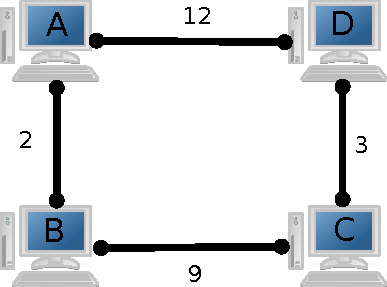
\includegraphics[scale=0.6]{img/algorithms/SAT_match}
%   \label{figure:sat_match:before}
% }\qquad\qquad
% \subfigure[(left) A jumps to B in order to match the logical topology to the
% physical. (right) State of the logical topology after the jump.] {
%   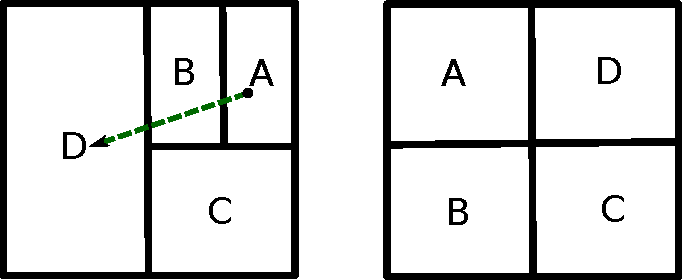
\includegraphics[scale=0.6]{img/algorithms/SAT_match2}
%   \label{figure:sat_match:after}
% }
% \caption{The SAT-Match algorithm.}
% \label{figure:sat_match}
% \end{figure}

\emph{SAT-Match}~\cite{RGJZ2004} defines an iterative process that 
adaptively changes the overlay network to ease the topology mismatch problem. 
It consists of a \emph{probing phase} in which a peer queries nearby nodes 
for distances and a \emph{jumping phase} in which the peer decides 
to change its neighborhood in order to reduce average neighbor distances. 
This process is performed iteratively
until no additional optimization is required; 
yet, the methods achieves optimization within a
sufficiently large scope.
%% VM This is used in other papers. Maybe we can put somewhere in the
% definition of Topology Mismatch Problem in the intro/background.
The notion of \emph{stretch} is used as the means for quantifying 
the \emph{topology match degree} of the constructed overlay;
stretch is defined as: 
$S = \bar{L_l}/\bar{L_p}$ where $\bar{L_l}$ is the average logical link
latency and $\bar{L_p}$ is the average physical link latency.
% 
% The \emph{probing phase} starts when the new-comer joins the \emph{DHT} 
% using the standard mechanism of the algorithm at hand. 
When a peer joins the \emph{DHT}, it starts 
its \emph{probing phase} by contacting the neighborhood with 
messages having small \emph{TTL=k}~\cite{jiang_lightflood_2008}. 
Recipients return information to the source and forward the message 
if not expired. 
After discovering its \emph{TTL}-$k$ neighborhood, 
the source measures \emph{RTT}-times, sorts them
and picks the two nodes with the smallest \emph{RTT}s.

During the \emph{jumping phase}, the source node calculates the 
stretch change to all its direct neighbours and to the direct neighbours
of the first peer that was selected in the probing phase, as if
the jump has been performed. 
Using heuristics, the node determines if the stretch
reduction is sufficient to perform the actual jump; 
otherwise, it selects the second peer from the probing phase 
and repeats the computation. If again, the
threshold is not met, then no jump is ultimately carried out.

Experimentation shows that \emph{SAT-Match} 
attains a $27\%$ stretch reduction over 
a landmark-enhanced \emph{CAN}-alternative.
This result shows that \emph{SAT-Match} 
may perform better than landmark binning in terms of the matching degree
of the logical to the physical networks.
\emph{SAT-Match} behaves as follows with respect to the stated $3$ criteria:
%%
% Figure~\ref{figure:sat_match} demonstrates the selective jump on an
% example topology.
%
%\paragraph{}
%Moreover the algorithm takes several issues into consideration in order to
%  further improve the resulted overlay. For example when multiple nodes try
% to jump simultaneously into a region, then the logical link brakes from one
% attempt may result in inaccurate computation of the gain factor, for an other.
% This situation is identified as \emph{contention} and the nodes use an
% exponential back-off algorithm to avoid it. An other problem is the
%unnecessary
% traffic incurred by the probing phase in a region that after several jumps
% has settled to a stable state. In these cases it is more likely for jump
% attempts to be proven worthless. The algorithm doubles the probing period of
% such nodes, every time a jump is not taken.
%
%\paragraph{}
%The authors claim that this continuously adaptive mechanism achieves global
%  topology matching optimization in a sufficiently large scope. This also
% secures the fast adaptation to frequent network changes. It also considered
% lightweight and can easily be embedded into current \p\ systems, as well
% as effectively combined with other techniques, such as landmark binning.
%%
%
% TODO: SOME DISCUSSION
%
% It is reported that,
% due to the selective jumps, SAT-Match achieves $40\%$ reduction in
% link stretch, and when used with the landmark binning (see
% Sec. \ref{sec:landmark_binning}), the reduction rate increases up to $60\%$.
% For dynamic environments, with frequent node arrival and leave, SAT-Match
% scales much better than Mithos, due to its self adaptation mechanism and
% selective jumps.
%%
\begin{center}
{\footnotesize
\begin{tabular}{ccc}
\emph{Efficiency} & \emph{Overhead} & \emph{Scalability} \\
\hline
% SAT-Match seems to outperform landmark binning in the sense of providing a
% higher grained differentiation of proximity, adding to the fact that
% SAT-match is fully distributed. Also to further enhance the efficiency it can
% work cooperatively with landmark binning itself.
% Security is compromised with arbitrary jumps!
high &
% distance probing and iterative computations add to the approach's overhead.
% Also the fact that the selective jumps are not always performed the added
% overhead to efficiency gained is not guaranteed in any configuration and
% circumstance.
medium &
% The self-adaptation nature of the algorithm and the selective jump mechanisms
% scale much better than, for example, Mithos. The test are on a relatively
% small amount of peers, thus, no safe conclusion can be made with respect to the
% algorithm's scalling performance.
medium
\end{tabular}
}
\end{center}

%%%%%%%%%%%%%%%%%%%%%%%%%%%%%%%%%%%%%%%%%%%%%%%%%%%%%%%%%%%%%%%%%%%%%%%%%%%%%%%%
%%%%%%%%%%%%%%%%%%%%%%%%%%%%%%%%%%%%%%%%%%%%%%%%%%%%%%%%%%%%%%%%%%%%%%%%%%%%%%%%
\subsection{Discussion on the Algorithms for Structured Architectures}
%%%%%%%%%%%%%%%%%%%%%%%%%%%%%%%%%%%%%%%%%%%%%%%%%%%%%%%%%%%%%%%%%%%%%%%%%%%%%%%%
%%%%%%%%%%%%%%%%%%%%%%%%%%%%%%%%%%%%%%%%%%%%%%%%%%%%%%%%%%%%%%%%%%%%%%%%%%%%%%%%

%% VM I commented out the following paragraph since it feels out of place
% (maybe better in the intro or background) or duplicated (from the intro or
% background).
%% 
% Structured \p\ network algorithms use a global distributed hash table or a
% prefix tree structure to uniquely lookup peers or their data in the overlay
% network. As all the data is kept within the overlay, each node behaves as a
% client and a server, therefore nodes join and leave according to rules
% determined by the integrity of the global data structure. The main advantage of
% the structured \p\ topology is that with the help of the global data structure,
% peers or their data can be found within the network even if there is only a
% single copy of that item present. However, each node join and leave creates
% maintenance overhead for the network due to updates required by the global data
% structure, and for networks with frequent node arrivals and departures, the
% overlay uses valuable network resources just to update the global structure.
% Nodes join the network by using a key value, which determines the location and
% the neighborhood of the new node within the network. However, assigning
% random key values to the newly inserted nodes creates non-optimal matching with
% the underlying physical network topology, therefore, increasing the overhead of
% the network even more. One solution for handling the topology mismatch problem
% is to consider the proximity of the peers when generating the key and joining
% the node to the network, so that nodes within the same network domains are
% selected as peers, or neighbors, during the overlay topology construction.

In this section, we have discussed research efforts 
trying to address the issue of inefficient network resource utilization 
manifested by network--topology mismatches in \emph{structured} \p-systems.
Based on the salient feature of outlined techniques
\cite{CDHR2002,CDCR2002,RSS2002}, we classify furnished solutions 
based on the following aspects:
\begin{enumerate}[\itshape i\upshape)]
  \item geographic-layout,
  \item proximity routing, and 
  \item proximity neighbor selection,
\end{enumerate}
%%
%%COM Added the following to mention the hybrid/combo methodologies
Similarly to unstructured approaches, most of the methods
reviewed in this section entail features from multiple of the above categories. 
For example, \cite{KLKP2008}~uses both proximity routing 
and proximity neighbor selection to achieve topology adaptation,
while \emph{LAPTOP} combines geographic--layout with
replication strategies to refine its results.
%%%
The heuristic nature of the suggested solutions opens them up 
to trade-offs which, in most cases, are 
highly affected by the application domain and the implementation itself.

%%AD Connection???  to the groups???
%%VM I like it. I put one similar to the unstructured part
In what follows, we place the surveyed structured \p-methods in 
the three categories mentioned above and which are formulated based 
on utilized proximity and geographic aspects.
With Table~\ref{structured:table}, we offer a comparative view
of the algorithms in a similar fashion to Table~\ref{unstructured:table}, 
to outline the key properties of each surveyed approach 
that helps differentiate techniques from
competitors~\footnote{The topics of topology adaptation, landmarking and
caching/replication are not further elaborated as they have been discussed 
in Section~\ref{section:unstructured}.}.
Finally, Figures~\ref{structured:plot:efficiency}, \ref{structured:plot:overhead}
and \ref{structured:plot:scalability} help with the pictorial comparison
of the algorithms' bahavior with respect to the three effectiveness
criteria we defined in Subsection~\ref{background:motivation}.

%%%%%%%%%%%%%%%%%%%%%%%%%%%%%%%%%%%%%%%%%%%%%%%%%%%%%%%%%%%%%%%%%%%%%%%%%%%%%%%%
\subsubsection{Geographic-layout} \label{section:geographic_layout}

%% In the \emph{geographic layout (GL)} category fall methods which practically
%This category consists of methods that 
%position physically nearby nodes together in the application space as 
%Figure~\ref{figure:geographic-layout} depicts. 
%This is accomplished by adjusting and maintaining the routing tables 
%of all involved peers by exploiting proximity information 
%that describe the overall geographic positioning of peers. 
%%AD I am not sure I follow the 1-line above...

%% VM: I reworded the above as below.
This category consists of methods that try to map the overlay id space on to
the physical one, as depicted in Figure~\ref{figure:geographic-layout}.
Routing tables of involved peers, are adjusted and maintained by exploiting
proximity information that describes the overall (geographic) positioning of
the participants. This comes in contrast to proximity routing and proximity neighbour
selection (discussed later on) where decisions are taken based on and effecting
a peer's nearby environment.

\begin{figure}[ht]
\centering
  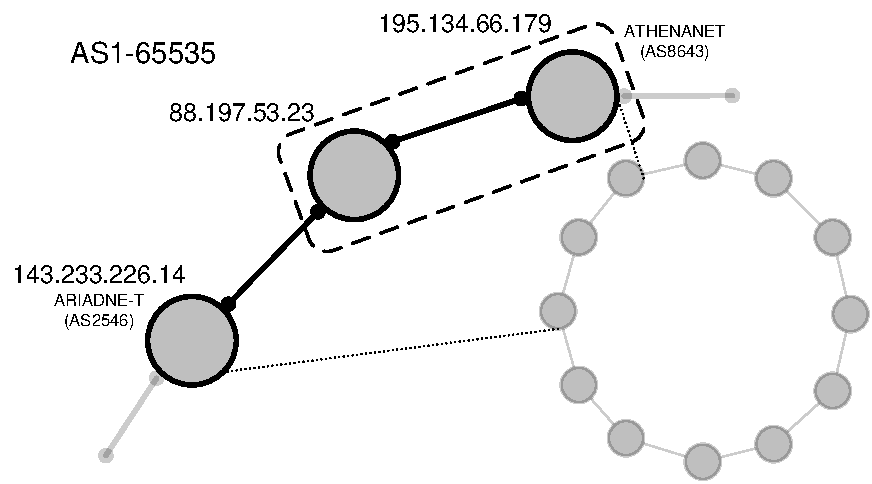
\includegraphics[scale=0.44]{img/pdf/geographic-layout.pdf}
\caption{Successive nodes in the overlay circle can be chosen to be from the
same or near autonomous systems (\emph{AS}).}
\label{figure:geographic-layout}
\end{figure}
%%
A number of the reviewed algorithms including 
\emph{Global Soft-State},
\emph{Mithos} and \emph{LAPTOP} resort to clustering close-by nodes in
order to reduce the network's average delay.
Landmark servers and \emph{RTT} measurements are two popular methods, which
can also be used in conjunction, to discover peers in physical proximity.
However, as already discussed, these
methods do not always yield reliable estimates for node positions over the
Internet. 
Landmark servers are not self-organizing and present maintenance
overhead. Moreover, to serve a structured \p--network with potentially 
tens of thousands or more 
% millions 
peers, multiple such servers are required to be distributed over the world, 
which is a difficult proposition per se.
\emph{RTT}s can measure the delay between peers, but their use constitutes a
greedy method that can result in sub-optimal overlay topologies;
the latter is especially true if nearby 
nodes happen to be connected through low bandwidth connections.

On one hand, approaches based on \emph{geographic layout} improve the query
efficiency of the system in general and are especially effective when applied
to \emph{CAN}-like implementations. On the other hand, they inherently undermine the
uniform distribution of peer identifiers. This is an important downside as it
creates hot-spots that hurt system scalability. 
Moreover, it adversely affects system availability as nearby nodes
are more likely to suffer collective failures~\cite{HY2007}.



%%%%%%%%%%%%%%%%%%%%%%%%%%%%%%%%%%%%%%%%%%%%%%%%%%%%%%%%%%%%%%%%%%%%%%%%%%%%%%%%
%
% TODO: Geographic Layout
%
%\begin{itemize}
% \item Geographic Layout\\
%The node IDs are assigned in such a way that nodes close by in the physical
%network topology, be close in the node ID space as well. Implementations that
%work relatively well with this approach have been incorporated into CAN. Nodes
%measure the RTT between themselves and a set of landmarks in order to match the
%CAN space as much as possible to the physical one. Unfortunately, the approach
%requires well known landmark servers and for that matter is  not fully
%self-organizing which can further lead to imbalanced node distribution. On
%other DHTs, such as Chord or Pastry, another problem emerges.  To gain fault
%tolerant properties, these protocols, replicate key-value pairs on neighboring
%(in the ID space) nodes. When a proximity-based node ID assignment has been
%used, the needed failure resilience is undermined by the fact that close by
%nodes are more likely to suffer collective failures.
%

%%%%%%%%%%%%%%%%%%%%%%%%%%%%%%%%%%%%%%%%%%%%%%%%%%%%%%%%%%%%%%%%%%%%%%%%%%%%%%%%
\subsubsection{Proximity Routing (PR)}

%This category of approaches % ({\emph{PR}) 
%does not require routing tables to be built using any
%knowledge about network proximity. 
%%%AD so if no knowledge is required what happens? How you go about 
%%%%
%%%AD I am not sure what the following sentence says... ;-) 
%On the other hand it exploits such knowledge
%to choose the best next hop when routing a message as can be seen in
%Figure~\ref{figure:proximity-routing}. 
%%%AD The above opening 2 sentences require re-calibration.. 
%%%

%% VM Rewrote above as below
This category of approaches use physical proximity knowledge to decide the best
next hop during routing. As shown in Figure~\ref{figure:proximity-routing},
maintenance of routing tables themselves is a separate process based only on the
system's DHT construction mechanism and overlay ID distribution.

\begin{figure}[ht]
\centering
  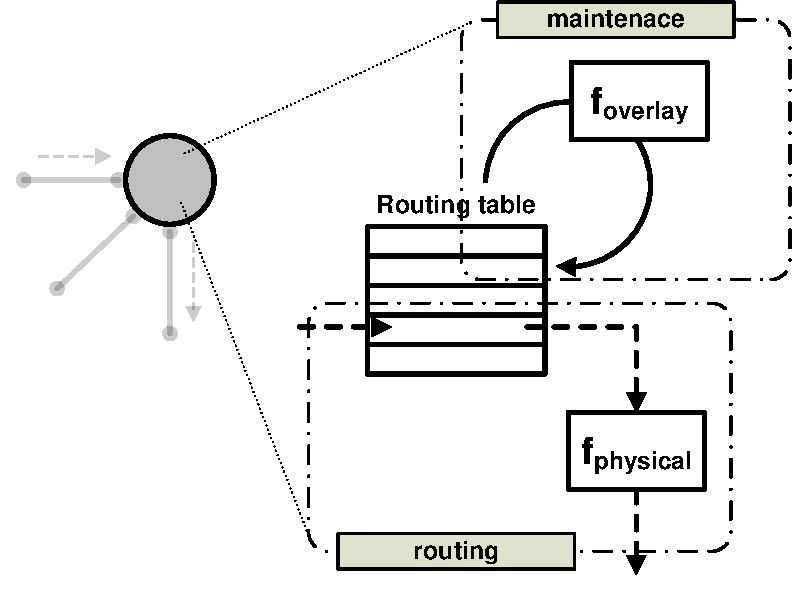
\includegraphics[scale=0.48]{img/pdf/proximity-routing.pdf}
\caption{Proximity routing takes proximity information into account during the
routing process.}
\label{figure:proximity-routing}
\end{figure}
%%
We reviewed an array of methodologies that strictly adhere to 
the tenets of this category such as \emph{Mithos} and
\emph{PChord} as well as others that function along with 
proximity neighbor selection such as \emph{DynaMO}.
%%
When \emph{PR}--based algorithms route messages, they try to balance between
choosing the node that will further progress the routing towards the
destination and picking the closest entry in the routing table
in terms of network proximity. 
%%AD just above in this section you have not clarified the way 
%%	routing tables get populated - u have to clarify this point 
%%	in order for the contrast here to be valid..
%%
%% VM Is the above now better with the rewording of the section's opening paragraph?
In the degenerate case, a system could use a greedy approach to select
only the lowest latency candidate peers during forwarding. That would to
longer, sub--optimal, paths to the destinations; thus imposing
extra stress to network resources. PR is also less
effective than geographical layout when applied to CAN--like implementations.
%%AD re-work carefully this segment...
%% VM how is it now?


% Moreover, the technique has been
% incorporated into a version of Chord causing an increase in the overhead of node
% joins and the size as well as maintenance cost of finger tables.

%
%\cite{dabek_cfs_2001} proposes a server selection scheme for the Chord DHT, on
%the domain of proximity routing selection. In \emph{CFS}, each node predicts
%the entire lookup latency as a function of the total number of nodes and the
%average overlay next routing peer. The problem is that it is very difficult to
%have a clear picture on the total number of nodes and the average hop latency
%from the local. This leads to rough estimations that consequently decreases
%overall performance.
%

%%%%%%%%%%%%%%%%%%%%%%%%%%%%%%%%%%%%%%%%%%%%%%%%%%%%%%%%%%%%%%%%%%%%%%%%%%%%%%%%
\subsubsection{Proximity Neighbor Selection (PNS)}

% \emph{Proximity Neighbor Selection (PNS)} 
Algorithms in this category use proximity data during routing table construction
and maintenance along the lines of Figure~\ref{figure:proximity-neighbour-selection}.
%%
\begin{figure}[hbft]
\centering
  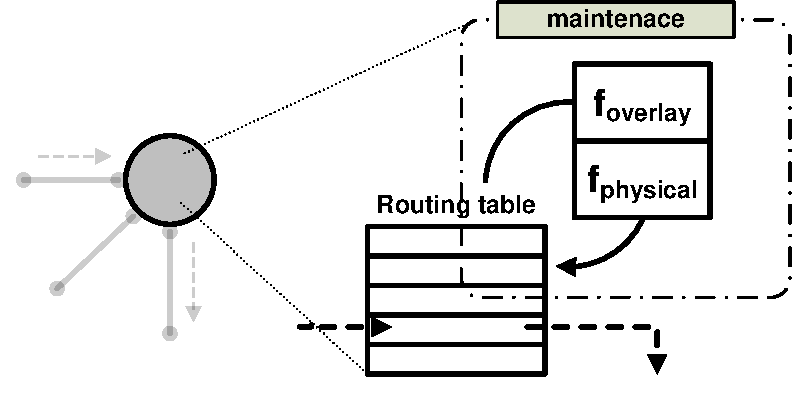
\includegraphics[scale=0.48]{img/pdf/proximity-neighbor-selection.pdf}
\caption{Proximity neighbor selection dictates that proximity is taken into
account during routing table maintenance.}
\label{figure:proximity-neighbour-selection}
\end{figure}
%%
The proximity information used is different from that of 
landmark-based systems described in Section~\ref{section:geographic_layout};
here, \emph{RTT} values between nodes (i.e., \emph{SAT-Match}) or 
\emph{IP} address prefixes (i.e., \emph{DynaMO}) % or \emph{Cone}) %%VM removing Cone from paper
are predominantly used to detect proximity. 
\cite{freedman_iploc_2005} states that $97\%$ of prefixes larger
than $24$ bits belong to a single geographical location. 
However, using a smaller number of bits creates less precise results 
and a larger number of bits may increase the burden in the network
and simultaneously reduce the possible number of neighbors. 
%%
Moreover, \cite{HLYW2005} argue that prefix--based approaches can
destroy the uniform distribution in the key space and do not work in
one-dimensional key space where the mapping is restricted to 
operate at the overlay.

Therefore, a careful selection is required in terms of
performance/accuracy trade-off. 
\emph{Tapestry}, \emph{Pastry}, and \emph{CAN} successfully incorporated
proximity neighbor selection into their methods. 
The routing protocol in \emph{Pastry} is based on longest node 
\emph{ID} prefix matching, while \emph{CAN} uses \emph{RTT} values to
detect nearby nodes. \cite{CDCR2002a} reports that proximity neighbor
selection is an effective proximity based method.
%%AD perhaps the ending of the previous segment should be used here...
%% VM: added below
In general, proximity neighbor selection is considered 
superior to proximity routing, however, simultaneous use of both
are also possible.

% \item Proximity Neighbor Selection\\
%Finally, the third approach, constructs the routing tables using proximity
%knowledge. Tapestry and Pastry's mechanisms of routing table
%maintenance try to minimize the distance to nodes appearing in a peer's routing
%table. Since routing is based on longest node ID prefix match, messages
%are gradually forwarded to nearby nodes at each routing step.
%\cite{castro_proximityp2p_2002} argues on how Pastry exploits proximity
%neighbor selection in order to create a scheme that is (more) location-aware
%compared to the other well-known DHTs (CAN, Chord).
%
%\end{itemize}
%
%{\sethlcolor{yellow}\hl{
%HA: Possible criteria: based on which protocol (eg Gnutella, CAN etc), peer
%selection (topology selection, cluster, cache etc), supports dynamic update,
%runtimes}}
%%\textbf{Algorithm} & \textbf{Overlay structure} & \textbf{Forwarding} &
%\textbf{Cache} & \textbf{Overlay optimization} & \textbf{Proximity information}
%& \textbf{Base protocol} & \textbf{Dynamic update} & \textbf{Runtime} \\
%
%
%{\sethlcolor{yellow}\hl{
%HA: Possible criteria2: Overlay optimization structure, base protocol (eg
%Gnutella, CAN etc), dynamic update, runtimes, scalability}}
%
%{\sethlcolor{yellow}\hl{
%HA: maybe add also the year of publication, and see if there is a pattern in
%terms of the method and the year??}}


%%%%%%%%%%%%%%%%%%%%%%%%%%%%%%%%%%%%%%%%%%%%%%%%%%%%%%%%%%%%%%%%%%%%%%%%%%%%%%%%
% \renewcommand\arraystretch{1.1}

\begin{landscape}
%\begin{figure}[h!]
\hspace{-3ex}
\begin{center}
\footnotesize
%\begin{tabular}{
\begin{longtable}{
m{2cm}
m{1cm}
m{1cm}
m{1cm}
m{1cm}
m{1cm}
m{1cm}
m{3cm}
m{5cm}
}
%|>{\columncolor[gray]{.7}}m{0.15\columnwidth}
%|>{\columncolor[gray]{.9}}m{0.05in}
%|>{\columncolor[gray]{.8}}m{0.05\columnwidth}
%|>{\columncolor[gray]{.9}}m{0.05\columnwidth}
%|>{\columncolor[gray]{.9}}m{0.05\columnwidth}
%|>{\columncolor[gray]{.8}}m{0.05\columnwidth}
%|>{\columncolor[gray]{.9}}m{0.05\columnwidth}
%|>{\columncolor[gray]{.8}}m{0.1\columnwidth}
%|>{\columncolor[gray]{.9}}m{0.1\columnwidth}
%|>{\columncolor[gray]{.8}}m{0.1\columnwidth+}
%|
%}
\caption[Summary table for structured algorithms]{Summary table for structured algorithms.} \label{structured:table} \\
\hline
%%%%%%%%%%%%%%%%%%%%%%%%%%%%%%%%%%%%%%%%%%%%%%%%%%%%%%%%%%%%%%%%%%%%%%%%%%%%%%%%
% first head
\rowcolor[gray]{.5}
\textbf{Algorithm / Paper} &
\textbf{Topology Adaptation} &
\textbf{Landmarking} &
\textbf{Proximity Routing} &
\textbf{Proximity Neighbour Selection} &
\textbf{Geographic Layout} &
\textbf{Caching / Replication} &
\textbf{Highlights} &
\textbf{Pros / Cons}\\
\hline
\endfirsthead
%%%%%%%%%%%%%%%%%%%%%%%%%%%%%%%%%%%%%%%%%%%%%%%%%%%%%%%%%%%%%%%%%%%%%%%%%%%%%%%%
% subsequent heads
\multicolumn{9}{c}%
{\tablename\ \thetable\ -- \textit{Continued from previous page}} \\
\hline
\rowcolor[gray]{.5}
\textbf{Algorithm / Paper} &
\textbf{Topology Adaptation} &
\textbf{Landmarking} &
\textbf{Proximity Routing} &
\textbf{Proximity Neighbour Selection} &
\textbf{Geographic Layout} &
\textbf{Caching / Replication} &
\textbf{Highlights} &
\textbf{Pros / Cons}\\
\hline
\endhead
%%%%%%%%%%%%%%%%%%%%%%%%%%%%%%%%%%%%%%%%%%%%%%%%%%%%%%%%%%%%%%%%%%%%%%%%%%%%%%%%
% foot
\hline \multicolumn{9}{r}{\textit{Continued on next page}} \\
\endfoot
%%%%%%%%%%%%%%%%%%%%%%%%%%%%%%%%%%%%%%%%%%%%%%%%%%%%%%%%%%%%%%%%%%%%%%%%%%%%%%%%
% last foot
\hline
\endlastfoot
%%%%%%%%%%%%%%%%%%%%%%%%%%%%%%%%%%%%%%%%%%%%%%%%%%%%%%%%%%%%%%%%%%%%%%%%%%%%%%%%
% data
\textbf{Global Soft-State} &
{\large \CheckedBox} &
{\large \CheckedBox} &
{\large \Square} &
{\large \Square} &
{\large \CheckedBox} &
{\large \Square} &
\begin{tabular}[l]{m{3cm}}
Hybrid landmark binning.\\
Probing scheme for proximity detection.\\
Strategic injection of proximity info around the network.\\
Subscription-notification system to dynamically adapt to network changes.
\end{tabular} &
\begin{tabular}[l]{m{5cm}}
+ Greatly reduces routing latency to far away nodes.\\
-- Host state maintenance.\\
-- Unable to identify nodes that are close to routers/gateways.\\
-- Its static nature sacrifices the self-organising attribute of DHTs.
\end{tabular}
\\
\hline
%%%%%%%%%%%%%%%%%%%%%%%%%%%%%%%%%%%%%%%%%%%%%%%%%%%%%%%%%%%%%%%%%%%%%%%%%%%%%%%%
\textbf{Mithos} &
{\large \Square} &
{\large \Square} &
{\large \CheckedBox} &
{\large \Square} &
{\large \CheckedBox} &
{\large \Square} &
\begin{tabular}[l]{m{3cm}}
Directed incremental probing.\\
Synthetic coordinates.
\end{tabular} &
\begin{tabular}[l]{m{5cm}}
-- Does not effectively manage dynamic peer arrival and leave.
\end{tabular}
\\
\hline
%%%%%%%%%%%%%%%%%%%%%%%%%%%%%%%%%%%%%%%%%%%%%%%%%%%%%%%%%%%%%%%%%%%%%%%%%%%%%%%%
\textbf{LAPTOP} &
{\large \CheckedBox} &
{\large \Square} &
{\large \Square} &
{\large \Square} &
{\large \CheckedBox} &
{\large \CheckedBox} &
\begin{tabular}[l]{m{3cm}}
Tree-based hierarchy.
\end{tabular} &
\begin{tabular}[l]{m{5cm}}
+ Reduces hops during message routing.\\
+ Minimal maintenance overhead.\\
-- Heartbeat approach incurs overhead even when not needed.
\end{tabular}
\\
\hline
%%%%%%%%%%%%%%%%%%%%%%%%%%%%%%%%%%%%%%%%%%%%%%%%%%%%%%%%%%%%%%%%%%%%%%%%%%%%%%%%
\textbf{Landmark Binning} &
{\large \Square} &
{\large \CheckedBox} &
{\large \Square} &
{\large \Square} &
{\large \CheckedBox} &
{\large \Square} &
Binning &
\\
\hline
%%%%%%%%%%%%%%%%%%%%%%%%%%%%%%%%%%%%%%%%%%%%%%%%%%%%%%%%%%%%%%%%%%%%%%%%%%%%%%%%
\textbf{Proximity in Kademlia} &
{\large \CheckedBox} &
{\large \Square} &
{\large \CheckedBox} &
{\large \CheckedBox} &
{\large \Square} &
{\large \Square} &
\begin{tabular}[l]{m{3cm}}
% Replacing XOR metric with a function that minimises the underlying cost.\\
% Clustering (MaxMind geolocation technology).
\end{tabular} &
\begin{tabular}[l]{m{5cm}}
+ Proximity routing works in Kademlia to improve connection locality.
\end{tabular}
\\
\hline
%%%%%%%%%%%%%%%%%%%%%%%%%%%%%%%%%%%%%%%%%%%%%%%%%%%%%%%%%%%%%%%%%%%%%%%%%%%%%%%%
\textbf{CHOP6} &
{\large \Square} &
{\large \Square} &
{\large \CheckedBox} &
{\large \Square} &
{\large \Square} &
{\large \Square} &
\begin{tabular}[l]{m{3cm}}
Ipv6 format exploitation.\\
Additional RTT information.
\end{tabular} &
\\
\hline
%%%%%%%%%%%%%%%%%%%%%%%%%%%%%%%%%%%%%%%%%%%%%%%%%%%%%%%%%%%%%%%%%%%%%%%%%%%%%%%%
\textbf{T2MC} &
{\large \Square} &
{\large \CheckedBox} &
{\large \CheckedBox} &
{\large \Square} &
{\large \Square} &
{\large \Square} &
\begin{tabular}[l]{m{3cm}}
Clusterting using traceroute logs.
\end{tabular} &
\begin{tabular}[l]{m{5cm}}
+ Prioritise interaction of peers and edge gateways.\\
-- Extended overhead.\\
-- Traceroute is sometimes disabled by ISPs.
\end{tabular}
\\
\hline
%%%%%%%%%%%%%%%%%%%%%%%%%%%%%%%%%%%%%%%%%%%%%%%%%%%%%%%%%%%%%%%%%%%%%%%%%%%%%%%%
\textbf{PChord} &
{\large \Square} &
{\large \Square} &
{\large \CheckedBox} &
{\large \Square} &
{\large \Square} &
{\large \Square} &
\begin{tabular}[l]{m{3cm}}
Maintenance of a proximity list.
\end{tabular} &
\begin{tabular}[l]{m{5cm}}
+ Dynamic maintenance of the proximity list.\\
+ Reduces routing costs.\\
+ Can constrain constly jumps in and out of network partitions.\\
+ Maintenance cost kept to a minimal (node join/leave heartbeat for lists)
\end{tabular}
\\
\hline
%%%%%%%%%%%%%%%%%%%%%%%%%%%%%%%%%%%%%%%%%%%%%%%%%%%%%%%%%%%%%%%%%%%%%%%%%%%%%%%%
\textbf{AChord} &
{\large \Square} &
{\large \Square} &
{\large \CheckedBox} &
{\large \Square} &
{\large \Square} &
{\large \Square} &
\begin{tabular}[l]{m{3cm}}
Exploits IPv6's anycast mechanism.
\end{tabular} &
\begin{tabular}[l]{m{5cm}}
+ Releaved from the bootstrapping process.\\
+ Easy to implement (just the additional neighbourhood table).
\end{tabular}
\\
\hline
%%%%%%%%%%%%%%%%%%%%%%%%%%%%%%%%%%%%%%%%%%%%%%%%%%%%%%%%%%%%%%%%%%%%%%%%%%%%%%%%
\textbf{Chord6} &
{\large \Square} &
{\large \Square} &
{\large \CheckedBox} &
{\large \Square} &
{\large \Square} &
{\large \Square} &
\begin{tabular}[l]{m{3cm}}
Exploits IPv6's hierarchical features.
\end{tabular} &
\begin{tabular}[l]{m{5cm}}
+ Reduces inter-domain traffic between ISPs.\\
+ Easily portable to other DHTs.\\
-- It cannot distinguish between close by domains in order to identify the best
next hop when an interdomain step must be taken.
\end{tabular}
\\
\hline
%%%%%%%%%%%%%%%%%%%%%%%%%%%%%%%%%%%%%%%%%%%%%%%%%%%%%%%%%%%%%%%%%%%%%%%%%%%%%%%%
\textbf{DHT-PNS} &
{\large \Square} &
{\large \Square} &
{\large \Square} &
{\large \CheckedBox} &
{\large \Square} &
{\large \Square} &
\begin{tabular}[l]{m{3cm}}
Grouping through synthetic coordinates.\\
Partitioning using a concentric cycle clustering scheme.
\end{tabular} &
\begin{tabular}[l]{m{5cm}}
-- It assumes uniform node distribution which is not always the case in a synthetic coordinate system.\\
-- Clustering nodes might be a single point of failure.
\end{tabular}
\\
\hline
%%%%%%%%%%%%%%%%%%%%%%%%%%%%%%%%%%%%%%%%%%%%%%%%%%%%%%%%%%%%%%%%%%%%%%%%%%%%%%%%
\textbf{Quasi-Chord} &
{\large \Square} &
{\large \CheckedBox} &
{\large \Square} &
{\large \CheckedBox} &
{\large \Square} &
{\large \Square} &
\begin{tabular}[l]{m{3cm}}
Geometric space coordinates (GNP)\\
Transformation of the coordinate space into 1-d Cantor space for easier mapping to the Chord hierarchy\\
Two finger tables (clockwise, anti-clockwise)
\end{tabular} &
\begin{tabular}[l]{m{5cm}}
-- Not fully distributed (GNP is landmark based).\\
-- Makes an indirect assumption of a maximum number of allowable hosts.\\
-- Doubles the required routing information which needs to be created and maintained.
\end{tabular}
\\
\hline
%%%%%%%%%%%%%%%%%%%%%%%%%%%%%%%%%%%%%%%%%%%%%%%%%%%%%%%%%%%%%%%%%%%%%%%%%%%%%%%%
\textbf{IPBC} &
{\large \Square} &
{\large \Square} &
{\large \Square} &
{\large \CheckedBox} &
{\large \Square} &
{\large \Square} &
\begin{tabular}[l]{m{3cm}}
IP address prefixes (16 bit for IPv4) to detect proximity.
\end{tabular} &
\begin{tabular}[l]{m{5cm}}
+ Prefix is stored in the DHT so the proximity identification becomes as easy as to query the prefix.\\
+ DHT maintenance mechanisms for both volunteer or falure departures of peers.\\
-- Performance/accuracy tradeoff in choosing the prefix length to be used.
\end{tabular}
\\
\hline
%%%%%%%%%%%%%%%%%%%%%%%%%%%%%%%%%%%%%%%%%%%%%%%%%%%%%%%%%%%%%%%%%%%%%%%%%%%%%%%%
\textbf{Cone} &
{\large \Square} &
{\large \CheckedBox} &
{\large \Square} &
{\large \CheckedBox} &
{\large \Square} &
{\large \Square} &
\begin{tabular}[l]{m{3cm}}
2-layer ID space.\\
Group concept for dividing nodes according to a common Chord id prefix.
\end{tabular} &
\begin{tabular}[l]{m{5cm}}
+ The first step of the routing scheme exploits proximity thus reducing message exchange costs.\\
-- Not fully distributed as it relies on landmarks.\\
-- Maintenance of three routing tables is needed.
\end{tabular}
\\
\hline
%%%%%%%%%%%%%%%%%%%%%%%%%%%%%%%%%%%%%%%%%%%%%%%%%%%%%%%%%%%%%%%%%%%%%%%%%%%%%%%%
\textbf{DynaMo} &
{\large \Square} &
{\large \CheckedBox} &
{\large \Square} &
{\large \CheckedBox} &
{\large \Square} &
{\large \Square} &
\begin{tabular}[l]{m{3cm}}
Random Landmarking (RLM).\\
Closest Neighbour Prefix Assignment (CPNA).\\
Making last hop as local as possible.
\end{tabular} &
\begin{tabular}[l]{m{5cm}}
+ Developed with mobile, ad-hoc networks in mind.\\
+ Evenly distributed IDs.\\
+ Dynamic landmarking is a fully distributed approach.\\
-- RLM imposes extra network stress especially to landmark nodes.\\
-- CPNA is a coarse-grained proximity approach.
\end{tabular}
\\
\hline
%%%%%%%%%%%%%%%%%%%%%%%%%%%%%%%%%%%%%%%%%%%%%%%%%%%%%%%%%%%%%%%%%%%%%%%%%%%%%%%%
\textbf{SAT-Match} &
{\large \Square} &
{\large \Square} &
{\large \Square} &
{\large \CheckedBox} &
{\large \Square} &
{\large \Square} &
\begin{tabular}[l]{m{3cm}}
Selective jumps to adjust peer positioning in the DHT.\\
Stretch reduction scheme.
\end{tabular} &
\begin{tabular}[l]{m{5cm}}
+ Continuously adaptive mechanism.\\
+ It can be considered lightweight.\\
+ Can coexist with other approaches (like landmarking).\\
+ Works sufficiently for large scopes as well as environments with high churn.\\
+ Compared to Mithos scales much better.\\
-- Contention situation in selective jump phase.\\
-- Probing phase incurs unnecessary traffic.
\end{tabular}
\\
\hline
%%%%%%%%%%%%%%%%%%%%%%%%%%%%%%%%%%%%%%%%%%%%%%%%%%%%%%%%%%%%%%%%%%%%%%%%%%%%%%%%
\textbf{Delay Aware P2P System} &
? &
? &
? &
? &
? &
? &
? &
?
\\
\hline
%%%%%%%%%%%%%%%%%%%%%%%%%%%%%%%%%%%%%%%%%%%%%%%%%%%%%%%%%%%%%%%%%%%%%%%%%%%%%%%%

% \hline
% \textbf{Global Softstate} &
% \textbf{Geographic layout} Uses first landmark clustering
% then measures RTTs to identify close nodes &  &  \\

% \hline
% \textbf{Mithos} &
% \textbf{Geographic layout} Uses nodes as topology landmarks and directed
% incremental probing to optimize topology & & Scales well as all
% operations are local ??? \\
% 
% \hline
% \textbf{Self-Adaptive Topology Matching} &
% \textbf{Proximity neighbour selection} Uses lightweight probing and
% selective jumps to optimize the topology & CAN &  Better than Mithos \\

% \hline
% \textbf{Delay Aware P2P System} & \textbf{} & & \\

% \hline
% \textbf{VERSION OF CHORD - DHT-PNS} &
% \textbf{Proximity neighbour selection} Uses Proximity Neighbour Selection and the Vivaldi
% system & Chord  &  \\

% \hline
% \textbf{MAY OMIT- VERSION OF CHORD - Quasi-Chord} &
% \textbf{Proximity based}  & Chord  &  \\

% \hline
% \textbf{LAPTOP} &
% \textbf{Geographic layout} Hierarchical overlay structure  &  & routing path length $\log{_d N}$,
% join/leave overhead $d\log{_d N}$ \\

% \hline
% \textbf{IP-Based Clustering} &
% \textbf{Proximity neighbour selection} Proximity neighbour selection based on longest common
% prefix of IP addresses &    &  \\

% \hline
% \textbf{CHOord considering Proximity on IPv6} &
% \textbf{Proximity routing} Uses IPv6 address format to provide proximity &  Chord
%  & Better than Chord \\

% \hline
% \textbf{Proximity in Kademlia} &
% \textbf{Proximity routing} Applies  proximity neighbour selection (PNS) and proximity route selection (PRS)
% to Kademlia & Kademlia &   \\

% \hline
% \textbf{Cone} &
% \textbf{Proximity neighbour selection} Uses proximity neighbour selection (PNS) & Chord  & Better than Chord \\

% \hline
% \textbf{DynaMO} &  &  &  \\
% 
% \hline
% \textbf{MAY OMIT-BADLY WRITTEN-PChord} &
% \textbf{Proximity based}  &  Chord  & \\
% 
% \hline
% \textbf{AChord} &  & & \\

% \hline
% \textbf{Chord6} &
% \textbf{Proximity routing} Uses IPv6 hierarchical address format to cluster
% topologically close nodes & Chord  &  \\

% \hline
\end{longtable}
\end{center}
\vspace{-2.5ex}
\vspace{-2.5ex}
%\label{fig:struct_compare_table}
%\end{figure}
 \end{landscape}


%%%%%%%%%%%%%%%%%%%%%%%%%%%%%%%%%%%%%%%%%%%%%%%%%%%%%%%%%%%%%%%%%%%%%%%%%%%%%%%%
%%%%%%%%%%%%%%%%%%%%%%%%%%%%%%%%%%%%%%%%%%%%%%%%%%%%%%%%%%%%%%%%%%%%%%%%%%%%%%%%
%                               STRUCTURED
%%%%%%%%%%%%%%%%%%%%%%%%%%%%%%%%%%%%%%%%%%%%%%%%%%%%%%%%%%%%%%%%%%%%%%%%%%%%%%%%
%%%%%%%%%%%%%%%%%%%%%%%%%%%%%%%%%%%%%%%%%%%%%%%%%%%%%%%%%%%%%%%%%%%%%%%%%%%%%%%%

%\pgfplotsset{width=7cm,compat=newest}
\onecolumn

%%%%%%%%%%%%%%%%%%% EFFICIENCY %%%%%%%%%%%%%%%%%%%
\begin{figure}[ht]
\centering
\resizebox{\textwidth}{!}{%
%\begin{landscape}
%\begin{center}
\begin{tikzpicture}
\begin{axis}[
  xbar,
  bar width=7pt,
  xlabel=\emph{Efficiency},
  ylabel=\emph{Algorithm},
  symbolic x coords={low, medium, high},
  symbolic y coords={
    SATMatch,
    3DO,
    DynaMOCNPA,
    DynaMORLM,
    %Cone,
    IPBC,
    QuasiChord,
    DHTPNS,
    Chord6,
    AChord,
    PChord,
    T2MC,
    CHOP6,
    ProximityInKademlia,
    %Landmark Binning,
    LAPTOP,
    Mithos,
    GlobalSoftState
  },
  every axis y label/.style=
    {at={(ticklabel cs:0.5)},rotate=90,anchor=near ticklabel},
%   x tick label style={rotate=45,anchor=east},
  xtick=data, ytick=data,
%   ymin=low,ymax=high,ytickmin=low,
  height=\textheight - 0.3cm,
  width=\textwidth,
  enlargelimits=0.05,
%  title=\emph{Efficiency} Pictorial Comparison of Structured Approaches.
]

\addplot[black,fill=gray!20, postaction={pattern=north east lines}]
table[x=EFFICIENCY,y=ALGORITHM]
{structured-plot.dat};

\end{axis}
\end{tikzpicture}
}
\caption{\emph{Efficiency} Pictorial Comparison of Structured Approaches.}
\label{structured:plot:efficiency}
\end{figure}
%\end{center}
%\end{landscape}

%%%%%%%%%%%%%%%%%%% OVERHEAD %%%%%%%%%%%%%%%%%%%
\begin{figure}[ht]
\centering
\resizebox{\textwidth}{!}{%
%\begin{landscape}
%\begin{center}
\begin{tikzpicture}
\begin{axis}[
  xbar,
  bar width=7pt,
  xlabel=\emph{Overhead},
  ylabel=\emph{Algorithm},
  symbolic x coords={low, medium, high},
  symbolic y coords={
    SATMatch,
    3DO,
    DynaMOCNPA,
    DynaMORLM,
    %Cone,
    IPBC,
    QuasiChord,
    DHTPNS,
    Chord6,
    AChord,
    PChord,
    T2MC,
    CHOP6,
    ProximityInKademlia,
    %Landmark Binning,
    LAPTOP,
    Mithos,
    GlobalSoftState
  },
  every axis y label/.style=
    {at={(ticklabel cs:0.5)},rotate=90,anchor=near ticklabel},
%   x tick label style={rotate=45,anchor=east},
  xtick=data, ytick=data,
%   ymin=low,ymax=high,ytickmin=low,
  height=\textheight - 0.3cm,
  width=\textwidth,
  enlargelimits=0.05,
%  title=\emph{Overhead} Pictorial Comparison of Structured Approaches.
]

\addplot[black,fill=gray!20, postaction={pattern=crosshatch}]
table[x=OVERHEAD,y=ALGORITHM]
{structured-plot.dat};

\end{axis}
\end{tikzpicture}
}
\caption{\emph{Overhead} Pictorial Comparison of Structured Approaches.}
\label{structured:plot:overhead}
\end{figure}
%\end{center}
%\end{landscape}

%%%%%%%%%%%%%%%%%%% SCALABILITY %%%%%%%%%%%%%%%%%%%
\begin{figure}[ht]
\centering
\resizebox{\textwidth}{!}{%
%\begin{landscape}
%\begin{center}
\begin{tikzpicture}
\begin{axis}[
  xbar,
  bar width=7pt,
  xlabel=\emph{Scalability},
  ylabel=\emph{Algorithm},
  symbolic x coords={low, medium, high},
  symbolic y coords={
    SATMatch,
    3DO,
    DynaMOCNPA,
    DynaMORLM,
    %Cone,
    IPBC,
    QuasiChord,
    DHTPNS,
    Chord6,
    AChord,
    PChord,
    T2MC,
    CHOP6,
    ProximityInKademlia,
    %Landmark Binning,
    LAPTOP,
    Mithos,
    GlobalSoftState
  },
  every axis y label/.style=
    {at={(ticklabel cs:0.5)},rotate=90,anchor=near ticklabel},
%   x tick label style={rotate=45,anchor=east},
  xtick=data, ytick=data,
%   ymin=low,ymax=high,ytickmin=low,
  height=\textheight - 0.3cm,
  width=\textwidth,
  enlargelimits=0.05,
%  title=\emph{Scalability} Pictorial Comparison of Structured Approaches.
]

\addplot[black,fill=gray!50, postaction={pattern=crosshatch dots}]
table[x=SCALABILITY,y=ALGORITHM]
{structured-plot.dat};

\end{axis}
\end{tikzpicture}
}
\caption{\emph{Scalability} Pictorial Comparison of Structured Approaches.}
\label{structured:plot:scalability}
\end{figure}
%\end{center}
%\end{landscape}

\twocolumn

